\documentclass{article}

\usepackage{polyglossia}
\setdefaultlanguage{english}
\setotherlanguage{sanskrit}
\usepackage{fontspec}
\newfontfamily\devanagarifont[Scale=MatchUppercase]{Kohinoor Devanagari}

\usepackage{graphicx}
\usepackage{subcaption}
\usepackage{float}
\usepackage[bottom]{footmisc}
\usepackage{enumitem}
\usepackage{hyperref}

\setlength{\parindent}{1.3em}
\setlength{\parskip}{0.7em}
\setlist{noitemsep}

\begin{document}

\begin{titlepage}
   \vspace*{\stretch{1.0}}
   \begin{center}
     \Huge\textbf{Vipassana for Hackers}\\
     \vspace{5cm}
     \large\textit{Steven Deobald}\\
     \large\textit{Version 1.6}\\
     \large\textit\today\\
     \vspace{5cm}
     \large\textit{Contributions by: Preethi Govindarajan, Mat Kelly, Liam Monahan}\\
   \end{center}
   \vspace*{\stretch{2.0}}
\end{titlepage}

\begin{center}
  \Huge{Target Audience}
\end{center}

Should you bother reading this paper? Not everyone associates themselves with the label ``Hacker''. It comes with a few well-known negative connotations so my first task is to quickly identify what is meant by ``Hacker'', since this paper is for these people.

My first exposure to the term ``hacking,'' outside of the late-80's imagery which became fodder for the 1995 film, was through my cousin Jennie. She is an Ecologist, a self-described ``Mud Scientist'', who most people would not associate with the term ``Hacker''. She visited MIT during her PhD to find the term extended to ``roof and tunnel hacking,'' an idea and practice which delighted her to no end. MIT or not, Jennie is a Hacker. Every Science is about exploration and discovery, and these are the concepts at the root of ``hacking.''

Carpentry, painting, gardening, the entire field of Genetics, baking bread, Philosophy, electronics, fashion, Psychology, health, writing, and bicycles. Almost any discipline can fall under the banner of ``hacking'' I'm using for this paper, since almost any discipline can (but does not necessarily) include the potential for two essential aspects of the Hacker Mentality: Rationality and Curiosity.

This is all that is required.

If you have ever enjoyed taking apart a computer or car, experimenting with bread recipes, researching and writing, pulling apart the semantics of your work, building something, rebuilding something, exploring a cave or abandoned construction site... I wrote this paper for you. If you enjoy any exploratory vocation or hobby you will almost certainly find Vipassana utterly fascinating. The reason is this: As acutely as a human being can disassemble a stereo, examine the slide of a microscope, or explore a cave, human beings have the capacity to disassemble, examine, and explore ourselves.

What may be even more fascinating, for the hacker, is the fact that by practicing Vipassana one can seemingly increase the capacity for rational thought and behaviour.

I have written this paper because, thus far, I have found the written and recorded material on the subject of Vipassana to fall into three broad categories:

Well-meaning Neuroscience papers which completely miss the mechanics of nervous-system-based meditation techniques and their core outcomes.
Descriptions of a ``silent meditation retreat,'' usually given by someone who has not attended a course. \cite{thenewsroom}
Descriptions of Vipassana from an individual and subjective perspective, usually given by someone who has attended one course. (``Oh my god! It was sooooo intense!'')

By using phrases like ``disassemble, examine, and explore ourselves'' I'm at the risk of sounding spiritual. This is the opposite of my intention. My intention is to pique curiosity in fellow hackers by explaining the biological mechanics of Vipassana, to the best of my ability and as I understand them. To curb the impression that this paper falls into the category of New Age Philosophy, I would like to take a moment to address what this paper is not.

\pagebreak

\begin{center}
  \Huge{What This Paper is Not}
\end{center}


This not an instruction manual. You will not learn Vipassana from reading this paper.

This is not a white paper. I am not a scientist. This is not science.

This is not an expert's treatise on the subject of nervous-system-based meditations, nor even an expert Vipassana meditator's description of the technique. I am not an expert. I have only attended four 10-day courses thus far. Each has been substantially different from the others.

This paper will endeavour to avoid falling into the trap of ``Buddhist Guys'' (a mildly derogatory term coined by a serious meditator friend of mine). You might be familiar with phrases commonly attributed to this archetype such as ``When the student is ready, the teacher will appear.'' Mysticism, mystery, and mystique are to be avoided. If I fall into this trap, email me: \href{mailto:steven@nilenso.com}{steven@nilenso.com}

This is not a discussion on ``spirituality'', for any definition of the term.

This is not a dissection of the administrative details of the course, though I will provide a brief overview of the course schedule.

This is not a description of past experiences, though I will use a few to highlight core effects of the technique.

This is not a comparison with other meditation techniques, though I will address other techniques for context. It is worth noting that there are a few meditation techniques labelled ``Vipassana'' and this paper deals specifically with Vipassana as taught by S.N. Goenka.

This is not an examination of Buddhist Philosophy and will exclude commentary or mention of the following concepts:

\begin{itemize}
  \item Siddhartha Gautama (The Buddha)
  \item Enlightenment
  \item Religion / Buddhism
  \item Prophecy / Prediction of the future
  \item Telepathy / ESP
  \item Reincarnation
  \item ``Energies''
  \item Kalapas
  \item Metta / Morality
  \item Sankharas / ``Impurity''
\end{itemize}

These last two bullet points are subject to one exception each.

\pagebreak

\begin{center}
  \LARGE{Morality's Exception: Lying}
\end{center}

A 10-day Vipassana course requires that all students take the standard \textit{5 Precepts} \cite{fiveprecepts}, as per Theravada. I do not recommend getting drunk, raping and murdering your fellow students, and stealing their belongings. However, the four precepts which forbid those behaviours are quite clearly external, making them components of course administration and therefore not applicable to this document.

Lying, however, is perhaps least interesting in its external form. As an educated adult, it is difficult to say anything at all without lying to some small degree. As one begins to systematically observe the nervous system, which is the basic mechanic of Vipassana, one finds that the brain and nervous system are acutely aware of even the tiniest untruth. If I tell myself I am feeling something which I am not (``my body is exploding into a billion tiny particles! my muscles are raging rivers of lava inside my body!'') the process of empirical and objective observation ends, and the process stops.

Therefore, the exception given to Lying (or the precept governing Lying) is because it actually prevents the technique from working, not because I have some particular crusade against lying.

\vspace{1cm}

\begin{center}
  \LARGE{Habit's Exception: Saṅkhāra}
\end{center}

The notion represented by the Pali word \textit{Saṅkhāra} can be split into two camps, in terms of its definition and use. The first, the notion that the body and mind contain ``impurities'' and that the objective of meditation is to rid the body-mind of such impurities, will be excluded from all discussion here. The second, more common use of the term ``Sankhara'' refers to ``conditioned phenomena'' or ``psychological dispositions''. The equivalent Hindi/Sanskrit word, \foreignlanguage{sanskrit}{संस्कार} (sanskaar) roughly translates in this context to ``mental impression''. This second definition will apply to this paper.

Here, we might choose a more specific term from Psychology: mental habits. Saṅkhāras, as far as this document is concerned, can be thought of as the ingrained habits of the brain and nervous system. Some concrete examples include liking (or disliking) the taste of olives, my body's ability to type at this QWERTY keyboard without consciously considering each keystroke, and the physical and emotional response I have to news of violence in my city of residence.

\pagebreak

\begin{center}
  \Huge{A Finger Pointing at the Moon}
\end{center}

The fundamental difficulty in any description of Vipassana is this: It is impossible to convey a description of Vipassana in terms known to someone who has not experienced it. During a Vipassana course this paradox is addressed using two metaphors: First, a story of a sighted brother explaining the concept of ``white'' to his blind brother. \cite{experiencethetruth} Second, the classic Indian story of blind men each describing an elephant and each producing a partial truth.

The first metaphor is a better framework for explaining the difficulty of writing about nervous system meditations. It is fundamentally impossible to express the experience of observing ``whiteness'' to an individual who is blind from birth. This person requires sight to understand. Similarly, it is fundamentally impossible to describe the effects of a nervous system meditation which alters perceptions and the interactions of the nervous system itself, since the nervous system (including the brain) ultimately form our entire experience.

The hacker community has been on the verge of this exploration for quite some time. The easiest and most recent examples of this are no doubt the works of Douglas Hofstadter. \textit{Gödel, Escher, Bach: An Eternal Golden Braid} captured the imaginations of the hacker community and grew from esoteric pub conversation piece to dinner party staple, around the same time as the term ``blogging'' evolved from portmanteau to an accessible part-time career for stay-at-home parents. The term ``strange loop'', coined in this book, has since become a mild obsession of philosophical and artistic computer scientists, linguists, and mathematicians, even inspiring the namesake software conference held in St. Louis. Hofstadter's more cohesive \textit{I Am a Strange Loop} tackles the problem of consciousness more succinctly. However, other than directing the reader to Zen\footnote{Zen is relevant because the practice of Zazen (Zen meditation) is a nervous-system-based meditation similar to Vipassana. The reason I do not discuss Zazen in detail or compare it to Vipassana in this paper is because Zazen, in my experience, is not systematic. The subject of inspection — the nervous system — remains, but Zen teachers tend to avoid explicit instruction, leaving the student to explore on her own. The outcomes, therefore, appear similar but watered down.} at multiple points, these books do not invite the reader to explore these concepts directly. There is no hacking. A thorough read of GEB or IAaSL is akin to reading all four volumes of Knuth's \textit{The Art of Computer Programming} \cite{taocp} without having ever touched a computer or to reading \textit{The Joy of Cooking} \cite{joyofcooking} cover to cover without having ever set foot inside a kitchen.

\pagebreak

\begin{center}
  \Huge{Computing Sidebar: LISP}
\end{center}

I will attempt to frame the self-exploration of nervous system meditations like Vipassana using one tool familiar to the Computer Science discipline: LISP. If you are neither a Computer Scientist nor a Linguist and have no interest in computer languages, feel free to skip to the next section.

Eric Raymond described the exercise of LISP mastery to be ``profound enlightenment'' \cite{hackerhowto} and while we can probably agree to ignore the hyperbole, there is something to be said about a language which begins as a calculus and nearly manages to escape formal grammar entirely. LISP has some very interesting properties:

\begin{itemize}
\item \textbf{Homoiconicity:} the language is represented in itself and code written in the language is understood by the language
\item \textbf{Metaprogramming:} the language can program itself and understand itself
\item \textbf{Self-mutation and self-replication:} a LISP program can inherently alter its own internal behaviour and easily write entirely new programs
\item \textbf{Recursion and trampolining:} mathematical functional recursion and mutual recursion between two functions are natural operations in LISP
\end{itemize}

Combined, these properties tend to blur the lines of compile time and run time, of code and data, of execution and interpretation. Decades ago, thanks to these ``strange loop'' properties of LISP, it was thought to herald the dawn of the Age of Artificial Intelligence. While that did not happen it left us with a fascinating building material: LISP appears to have no upper-bound. It is ``turtles all the way up.'' LISP is not ``turtles all the way down'', as some would describe it. Even if written on a LISP Machine (a computer which executes LISP directly rather than transforming LISP into machine-level instructions), there are still paths of wires and electrons which need to be dealt with. These are not written in LISP.

Vipassana would appear to be ``turtles all the way down'' in precisely this sense. Vipassana is the process of digging through your consciousness using consciousness itself. At no point do you reach the machine beneath the machine: ``Aha! I found it! The Consciousness Machine. Now I can do away with the meditation and just read the manufacturer's open specification and I'm sorted.'' \textit{The machine at the bottom of your consciousness is a strange loop}. Having a look at this strange loop is a lot more fun than reading about it.

\pagebreak

\begin{center}
  \Huge{Course Structure}
\end{center}

For those unfamiliar, I will briefly overview the rules of the course. During the course you are not permitted books, phones, talking, looking people in the eye, touching, making sounds, snacks, music, or writing implements.

Put more succinctly, your activities will include: Eat, sleep, poop, bath, meditate.

That's it.

Meditation will consume approximately ten to eleven hours per day. All courses the world over are free and volunteer-run. Material goods are provided for by donations from previous students.

\pagebreak

\begin{center}
  \Huge{Suspending Disbelief}
\end{center}

Before explaining the mechanics and outcomes of Vipassana, I must request that you suspend disbelief about three items for the duration of the paper.

\vspace{1cm}
\begin{center}
  \LARGE{1. Meditation is a thing}
\end{center}

For the purposes of this document, understand ``meditation'' to mean a single point of awareness with unwavering focus. ``Unwavering focus'' means that we can hold sustained attention on this single point (whatever it may be) without getting distracted by thoughts of our taxes, what's for lunch, or that really persistent itch on our ear.

What I mean by this is that mental exercises exist which can take consciousness beyond ``flow'', ``calm'', or ``elated'' states of mind caused by activities one might describe as ``meditative'' rather than ``meditation''. Biochemical responses to hallucinogens fall on the same side of the spectrum, though they may appear momentarily insightful.

I have drawn my personal spectrum for sample activities in Figure~\ref{fig:meditation-spectrum-1}.

\begin{figure}[H]
  \centering
  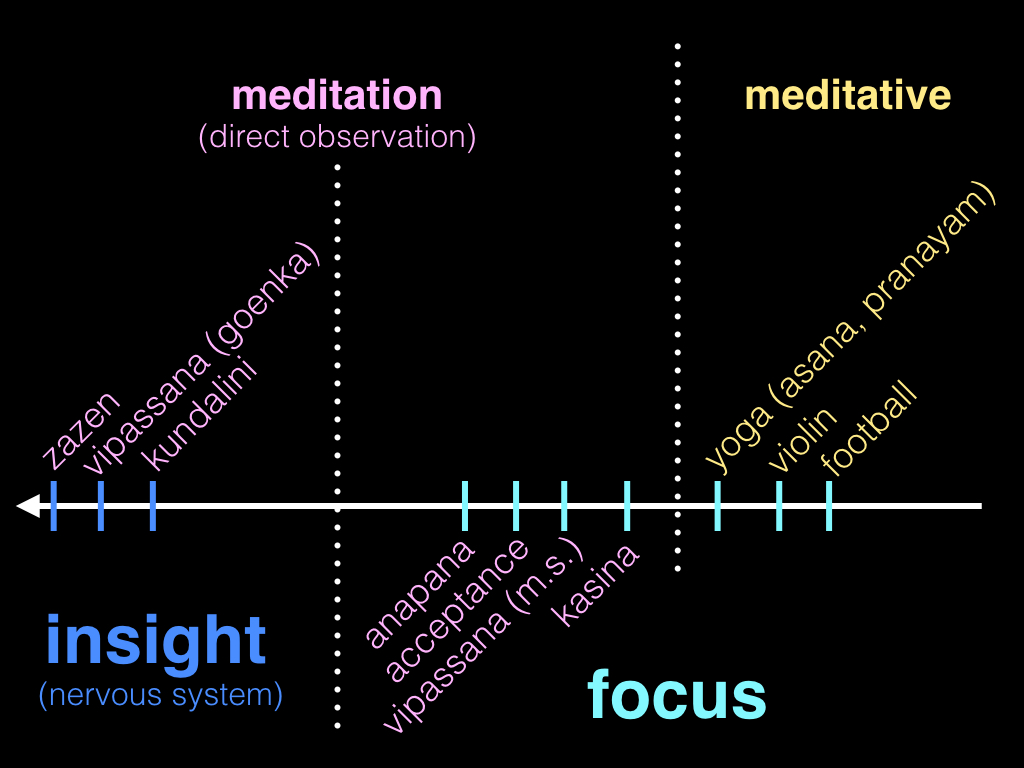
\includegraphics[width=11cm]{images/meditation-spectrum-1.jpeg}
  \caption{Sample meditation/meditative spectrum.}
  \label{fig:meditation-spectrum-1}
\end{figure}

For the purposes of this paper, we will keep all notions of ``mindfulness'' in the ``meditative'' camp, on the right. Mindfulness is not meditation. This paper will be discussing only two practices from this list: Anapana and Vipassana. An illustrated definition of ``awareness'' and ``attention'' follows, in the section entitled ``On Attention''.

\begin{figure}[H]
  \centering
  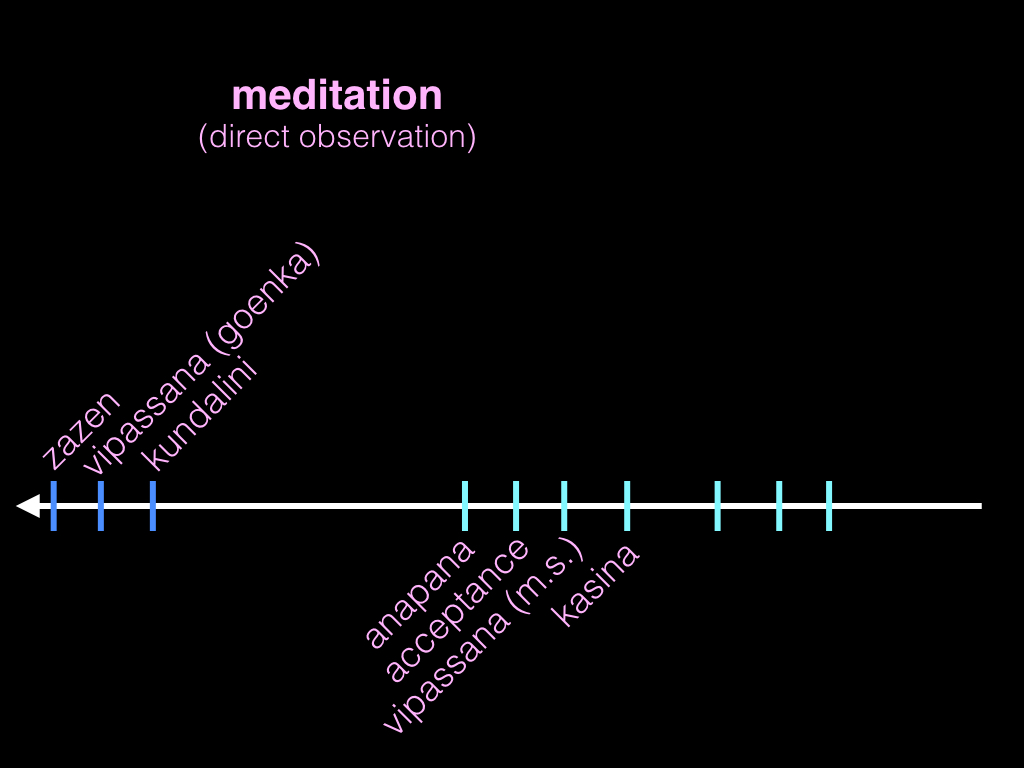
\includegraphics[width=11cm]{images/meditation-spectrum-3.jpeg}
  \caption{Sample meditation spectrum.}
  \label{fig:meditation-spectrum-3}
\end{figure}

\vspace{1cm}
\begin{center}
  \LARGE{2. Your brain and nervous system have}\\
  \LARGE{a tight feedback loop}
\end{center}

When we say ``tight feedback loop'', this means the brain and nervous system are tied together in a feedback loop faster and tighter than you could ever imagine without experiencing it directly.

We all know the classic examples of connectivity between the brain and nervous system: A child touches a hot stove and retracts her hand. A pubescent boy sees a boy or girl he is attracted to and feels ``butterflies in his stomach'' so intense he vomits. Despite healthy diet and exercise, a high-strung individual suffers from stomach ulcers.

These examples all exist on a gross level, coarse-grained enough that we can identify them externally and even give them names like ``butterflies''. However, your nervous system is interacting with your brain at every conceivable level. No matter how small, you do not have a thought or emotion emerge in your consciousness (or unconscious) without a physical sensation accompanying it. You do not feel physical sensation, consciously or subconsciously, without an accompanying thought or emotion. This interaction is continuous.

Unless you have tried a meditation system with the nervous system as its meditation object, you have almost undoubtedly not experienced this.

\vspace{1cm}
\begin{center}
  \LARGE{3. Dissolution of the body is a thing}
\end{center}

This will be the most difficult of the three. ``Dissolution of the body,'' though strange-sounding at first, does not fall into the categories where we would normally place magic, levitation, or ESP. The term simply refers to our capacity to see through our entire body.

As we investigate this concept, it seems increasingly reasonable in conjunction with points \#1 and \#2. If we can narrow our attention down to anything we can perceive and what we choose to perceive with our brain and nervous system in tandem is a narrow part of the body, surely if we sustain attention on that part for long enough we will start to see it clearly.

Normally, our attention on our body is almost entirely external: my hands on this keyboard, the itch on my ear, my butt in this chair. I don't tend to spend a lot of energy focused on the sensations provided to my brain by my gallbladder or my stomach unless I have a painful gallstone or I am experiencing acute hunger. Physical sensations provided to our awareness by the nervous system for the internals of the body are largely hidden from us — but they can be unearthed and explored.

I should note here that in four courses I have not felt the precise shape of my gallbladder or stomach at any point. I have ``seen'' the shape of my bones in my fingers, shoulders, chest, and pelvis. I have witnessed the rush of blood squooshing through my cardiovascular system (near the surface) with terrifying clarity. I have enough anecdotal evidence to say that it appears this process does work and can be extended to our deepest internal organs and the spinal cord.

To help visualize what I mean, a sample spectrum of sensations from the gross or obvious to the curious and subtle might look like the figure on the following page.

\begin{figure}[h]
  \centering
  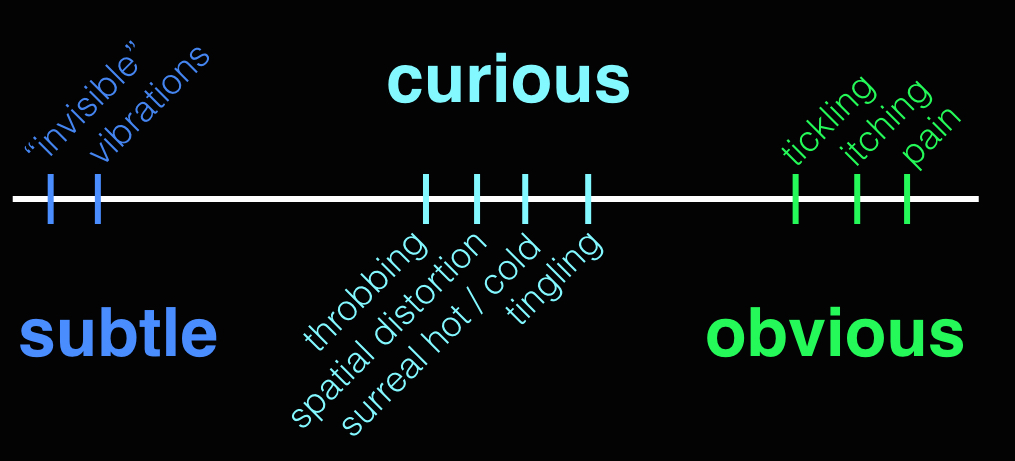
\includegraphics[width=\linewidth]{images/sensation-spectrum.jpeg}
  \caption{Sample sensation spectrum.}
  \label{fig:sensation-spectrum}
\end{figure}

As the field of sensation progresses to the left, the sensations felt become increasingly difficult to describe. ``Surreal hot / cold'' refers to sensations of temperature we wouldn’t normally consider possible: our muscles either on fire or freezing solid. ``Spatial distortion'' refers to complete alterations of spacial presence — the partial or complete replacement of one’s normal sense of proprioception. This may include reorientation in space (``I was upside-down!'') or the feeling that one is gigantic or tiny or that any one body part has one of these or other distorted qualities.

``Throbbing'' refers to thick, heavy, slower vibrations; these are often felt rhythmically and this rhythm accelerates until the sensation is described as a ``vibration''. Beyond vibration is the ``invisible'', where a particular body part is no longer seen and a deeper part of the body is experienced directly. The first such example in most cases tends to be the skin, since the external surface of the body is the first part of the nervous system the course instructions ask the meditator to focus on. Beyond this the meditator may find muscle tissue, bones, the cardiovascular system, or something else entirely. Usually by the point in the course when a meditator has dissolved her own skin to her attention the sensations become extremely difficult to identify and label so ``something else entirely'' is likely to be the most common case.

The sample spectrum above is missing many, many sensations. I also feel it necessary to call out that the spectrum is not serial; although I have felt ``vibrations'' and seen deeper than skin level, I have certainly not experienced all the sensations possible in the spectrum. However, the diagram hopefully provides a reference point for the type of readily-accessible sensations which Vipassana begins with (on the right) and the types of sensations (or absence of sensation) which will convince a person that complete dissolution of the body not only possible but an entirely natural process.


\pagebreak

\begin{center}
  \Huge{Virtual Reality}\\
  \Huge{and}\\
  \Huge{The Matrix Paradox}
\end{center}

The following section will require some visual assistance, for which I will use the same slides I used in the talk which corresponds to this paper. An unmodified slide is seen here in Figure~\ref{fig:michael-abrash-senses}.

\begin{figure}[h]
  \centering
  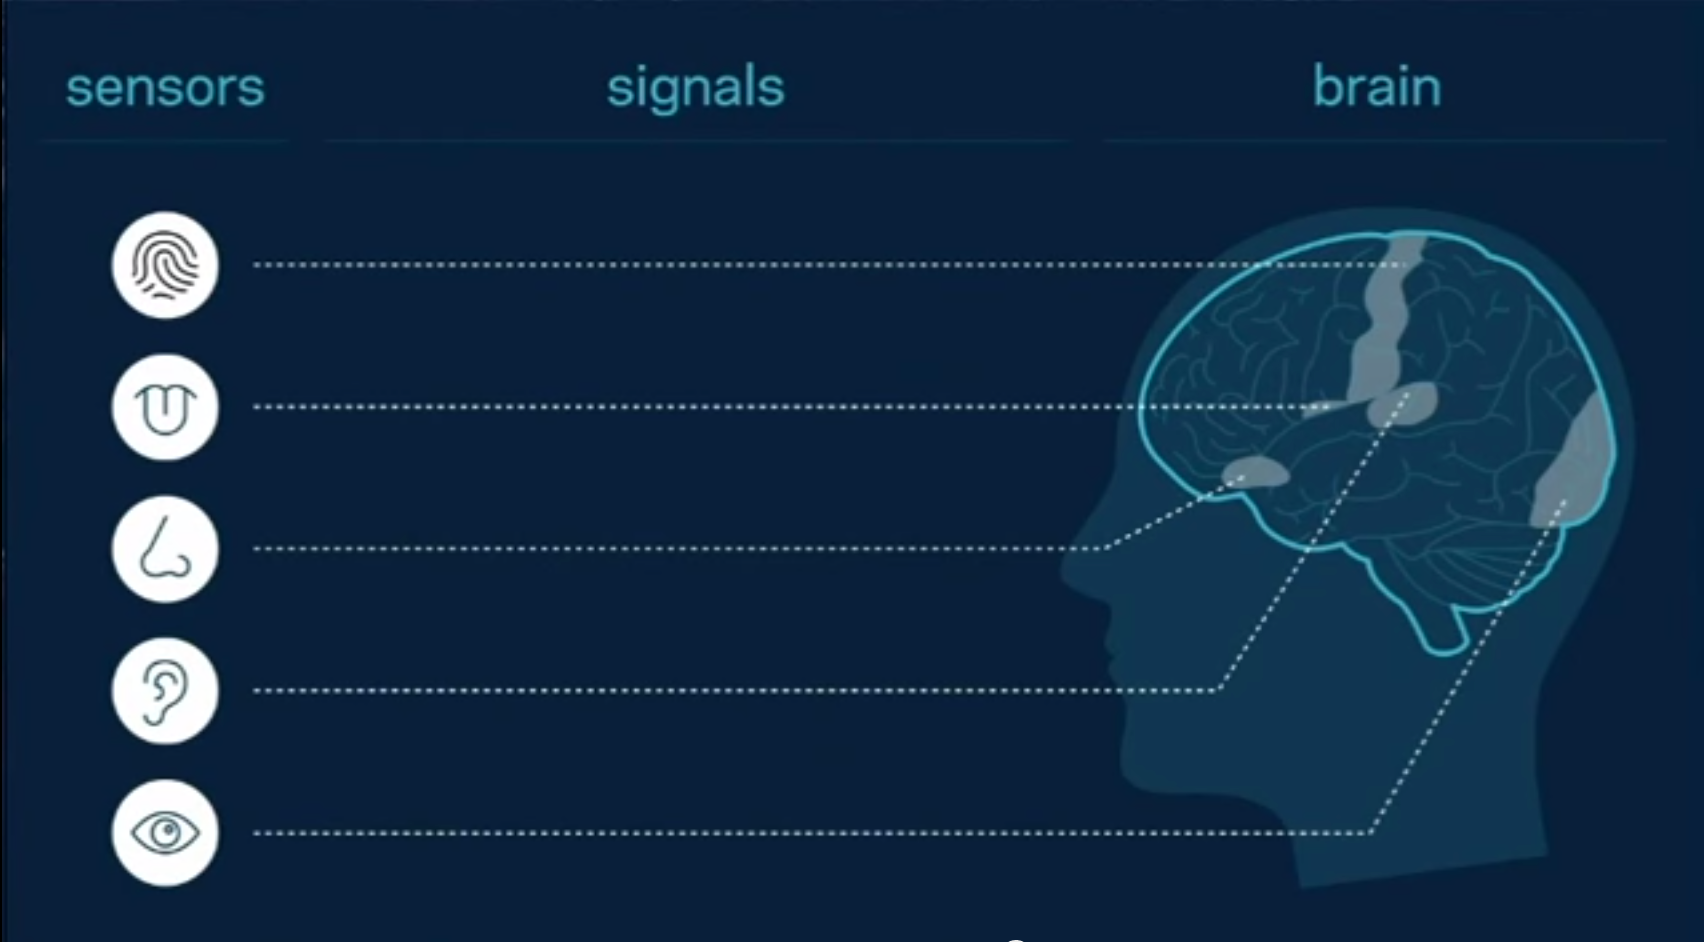
\includegraphics[width=\linewidth]{images/michael-abrash-senses.png}
  \caption{Traditional 5-sense brain mapping.}
  \label{fig:michael-abrash-senses}
\end{figure}

This image is taken from a talk by Michael Abrash, Chief Scientist of the Oculus VR team, at a talk he gave at the Facebook F8 Summit in 2015. \cite{abrashvr} I'm using this slide because it's nicely laid out and because it is incomplete.

Abrash discusses the nature of the ``Matrix Paradox'' (more commonly known as the \textit{Simulation Hypothesis} \cite{simulationhypothesis}) as simply the right neurons firing to simulate any particular environment. ``How do we know we are not in the matrix?'' The question is valid, but the diagram is missing a great deal of sensory input. Figure~\ref{fig:michael-abrash-senses-extended} is a slightly better model of reality.

\begin{figure}[h]
  \centering
  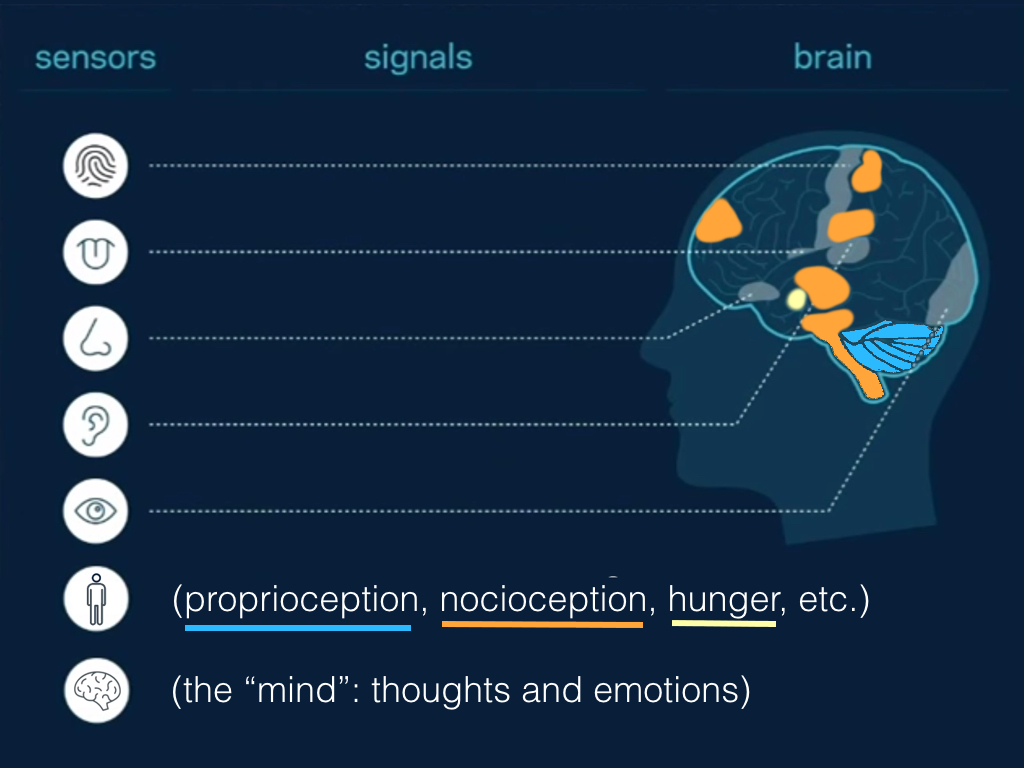
\includegraphics[width=\linewidth]{images/michael-abrash-senses-extended-attached.jpeg}
  \caption{A more complete, 7-sense brain mapping.}
  \label{fig:michael-abrash-senses-extended}
\end{figure}

Though a classic sense diagram such as Mr. Abrash's might describe proprioception \cite{ramachandranbrainfunction, proprioception}, nocioception \cite{nocioception}, and hunger \cite{fmrihunger} as physical ``feeling'', they are definitively not a subset of ``touch'', as they correspond to entirely different activity in the brain. Touch is strictly an external sense dealing with skin. These are internal senses.

A brain diagram describing The Matrix Paradox is complete only when we map all senses to the brain. I have not, since I haven't named them all. In fact, neurobiology does not yet have names for all sensory input, making such an exercise exceedingly difficult. Proprioception is clearly associated with the cerebellum and hunger is clearly associated with the hypothalamus. Nocioception, however, is a bit more nuanced with regard to the brain's reception of thermal, mechanical, and chemical information — and whether or not the activity is inbound, outbound, conscious, or unconscious. However, assuming all nervous system activity does have corresponding brain activity, one could theoretically map out the Matrix Paradox on the brain as Abrash has started. It seems likely such a diagram would highlight all parts of the entire brain.

On that note, I feel I should introduce an absolutely fantastic RadioLab episode (\textit{Where Am I?} \cite{whereami}) which addresses this topic of ``other senses'' from the perspectives brought by modern Neuroscience. On the topic of lacking proprioception:

\begin{quote}
  \textbf{We have words like `deaf' and `blind'. We do not have words for being deaf or blind to one's own body.}
\end{quote}

In the Matrix, perhaps this is either a bug or a feature flag.

Now that we have our diagram for visualizing the use of our senses, we can address them in terms of various altered mental states. Before we get there, however, we will try to come up with a meaningful visual definition of ``attention'' or ``awareness'' with respect to our senses.


\pagebreak

\begin{center}
  \Huge{On Attention}
\end{center}

The funny thing about Vipassana is that you are doing it already... you're just terrible at it. Vipassana is the inspection of one's own nervous system with narrowly-focused attention but the precision of this focus is not prescribed by the instruction given for the technique. ``As narrow as possible'', perhaps, but in day to day life a normal person cannot possibly narrow her attention to the size of a fingertip. Your attention is, in part, already on your nervous system, with some degree of focus. To the extent that it is, you are doing Vipassana.

If your attention is not directed at your nervous system, where is it? Let's look at three environmental examples which can help us highlight our senses and our awareness within them.

\pagebreak

\begin{center}
  \LARGE{Example 1:}\\
  \LARGE{A bustling restaurant}
\end{center}


\begin{figure}[h]
  \centering
  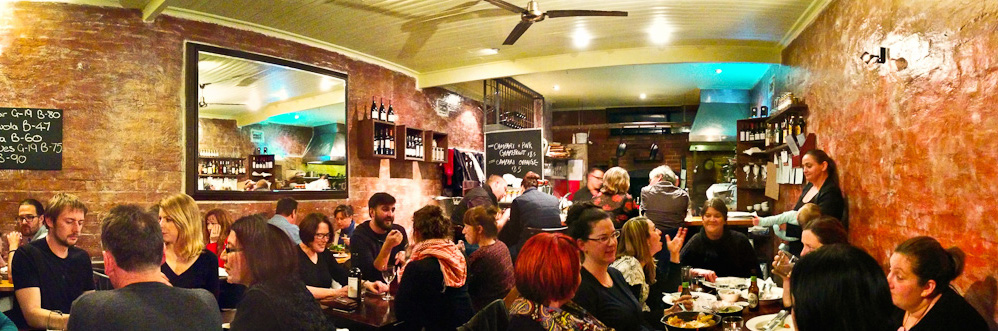
\includegraphics[width=\linewidth]{images/attention1-restaurant.jpg}
  \caption{A bustling restaurant.}
  \label{fig:bustling-restaurant}
\end{figure}

...and a corresponding sense map something like this:

\begin{figure}[h]
  \centering
  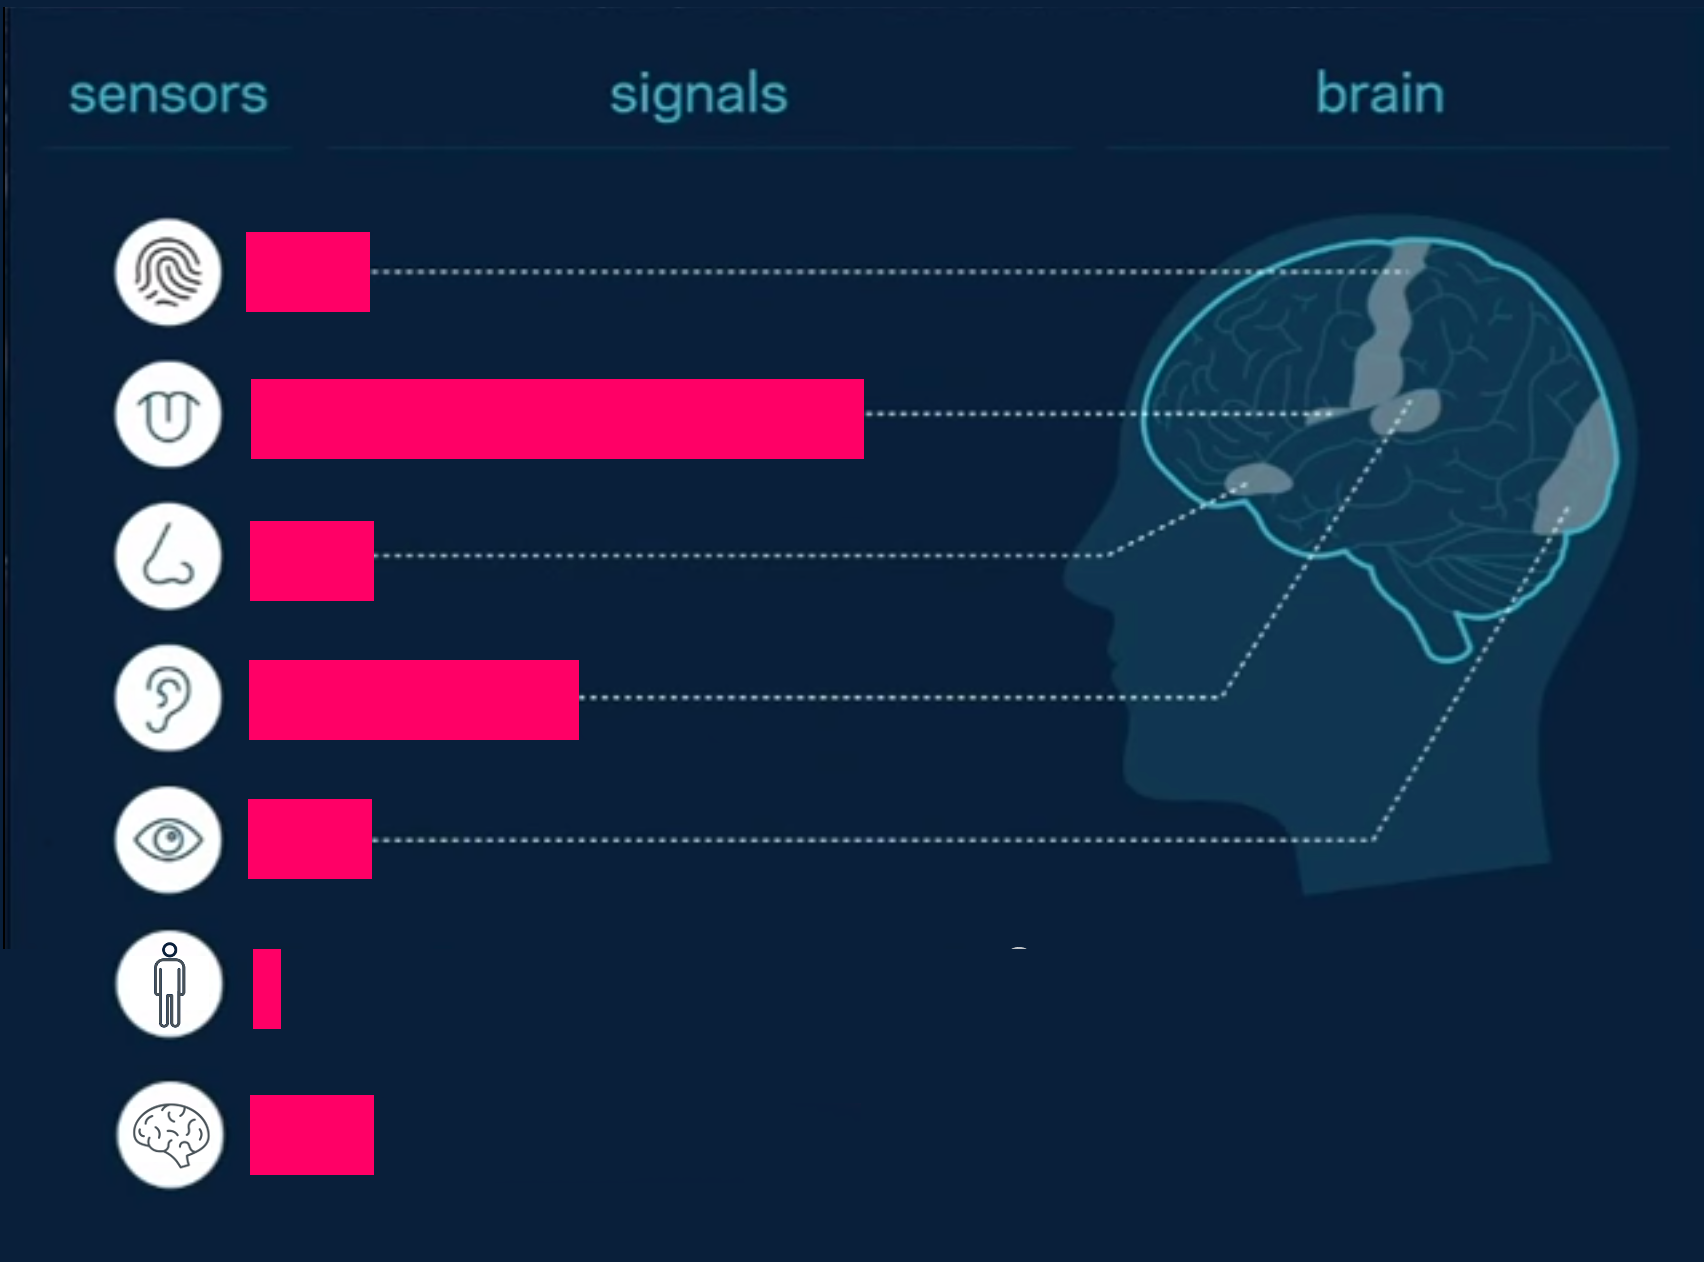
\includegraphics[width=10cm]{images/ma-noisy-restaurant.png}
  \caption{Sense map of a bustling restaurant.}
  \label{fig:sense-map-bustling-restaurant}
\end{figure}

Assuming we've just placed food in our mouths, our sense of taste is going off like crazy, we're hearing a lot of scattered sound around us, and we're also sufficiently distracted by most of our other senses. Note that we are probably paying very little attention to the internal senses.

\pagebreak

\begin{center}
  \LARGE{Example 2:}\\
  \LARGE{A sensory deprivation tank}
\end{center}

\begin{figure}[h!]
  \centering
  \begin{subfigure}[b]{0.48\linewidth}
    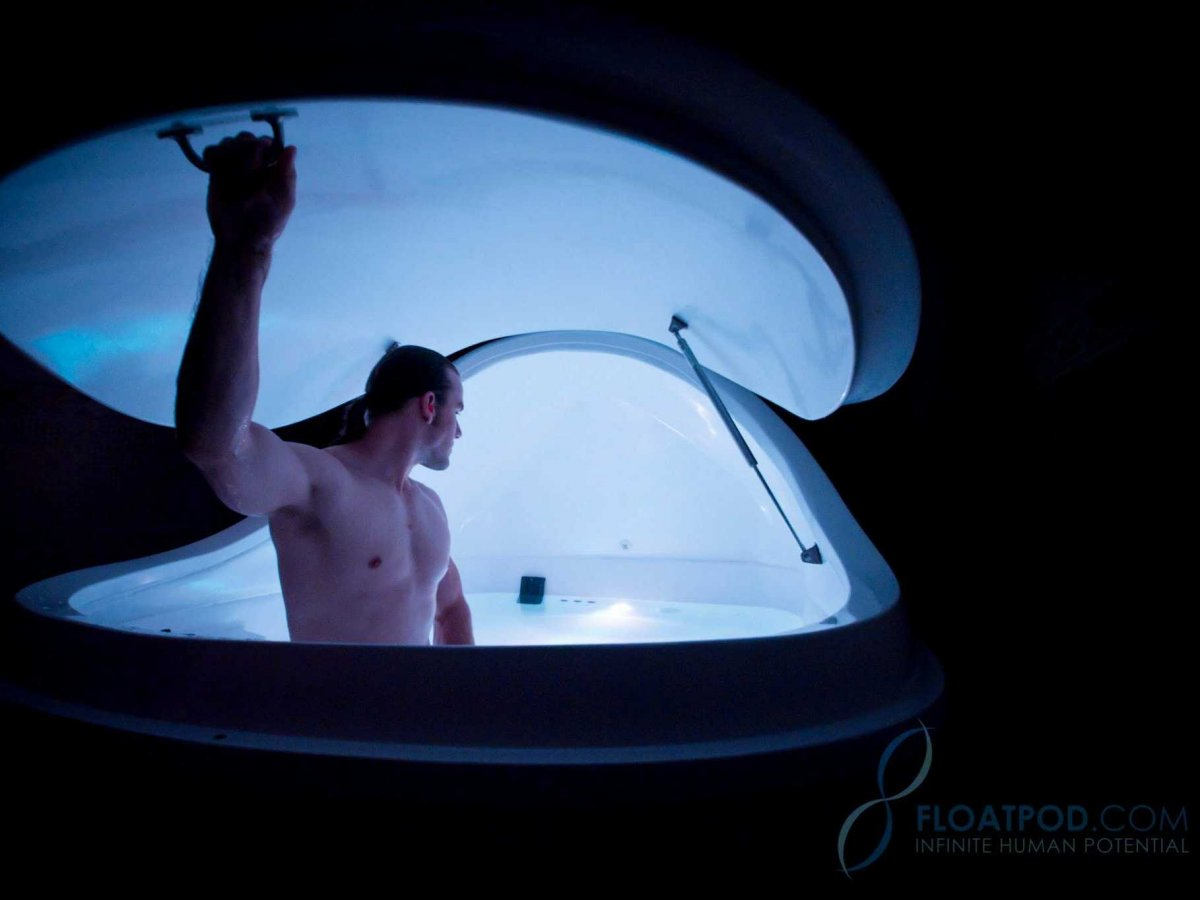
\includegraphics[width=\linewidth]{images/attention2-tank.jpg}
  \end{subfigure}
  \begin{subfigure}[b]{0.48\linewidth}
    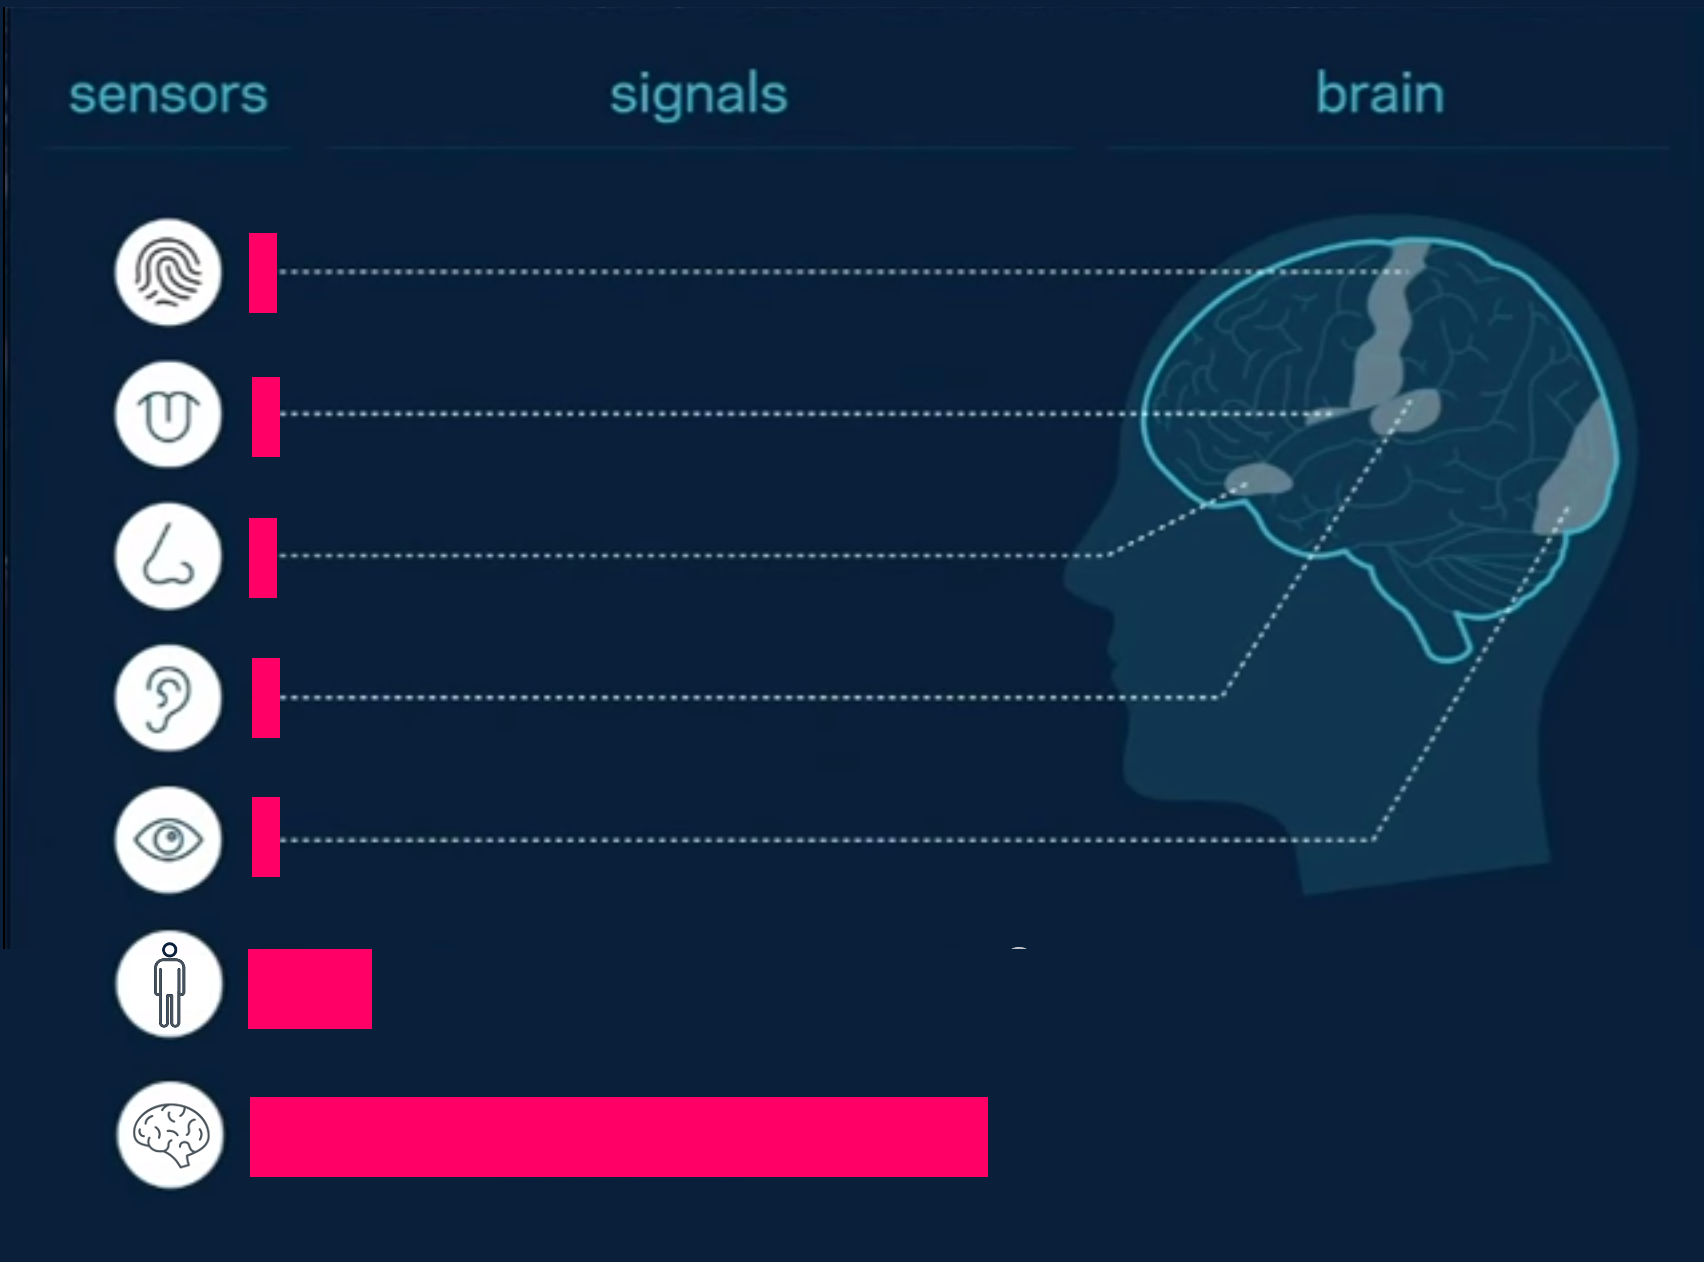
\includegraphics[width=\linewidth]{images/ma-sensory-deprivation-tank.png}
  \end{subfigure}
  \caption{A sensory deprivation tank and corresponding sense map.}
  \label{fig:sensory-deprivation-tank}
\end{figure}

Here, the classic 5-sense model fails us, since sensory deprivation only deprives us of these 5 senses. When Neo is first exposed to the reality of The Matrix, the pods which imprison the humans loosely resemble such sensory deprivation tanks, which is reason enough to believe that we are not in that matrix. As anyone who has ever entered a sensory deprivation tank knows, it is not like being in a coma. The mind is still very active and it may actually help in causing someone to pay attention to their internal senses.


\pagebreak

\begin{center}
  \LARGE{Example 3:}\\
  \LARGE{An anechoic chamber}
\end{center}

\begin{figure}[h!]
  \centering
  \begin{subfigure}[b]{0.48\linewidth}
    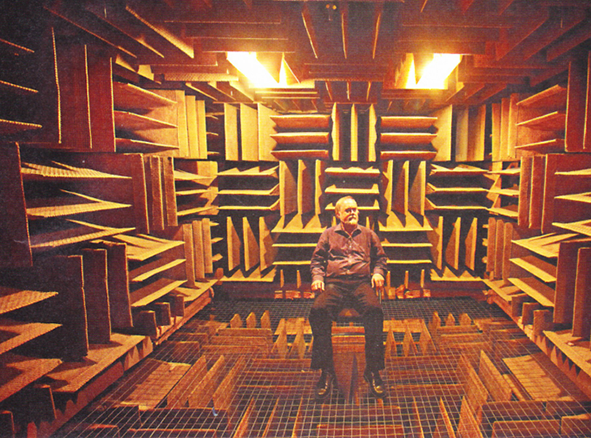
\includegraphics[width=\linewidth]{images/attention3-chamber.png}
  \end{subfigure}
  \begin{subfigure}[b]{0.48\linewidth}
    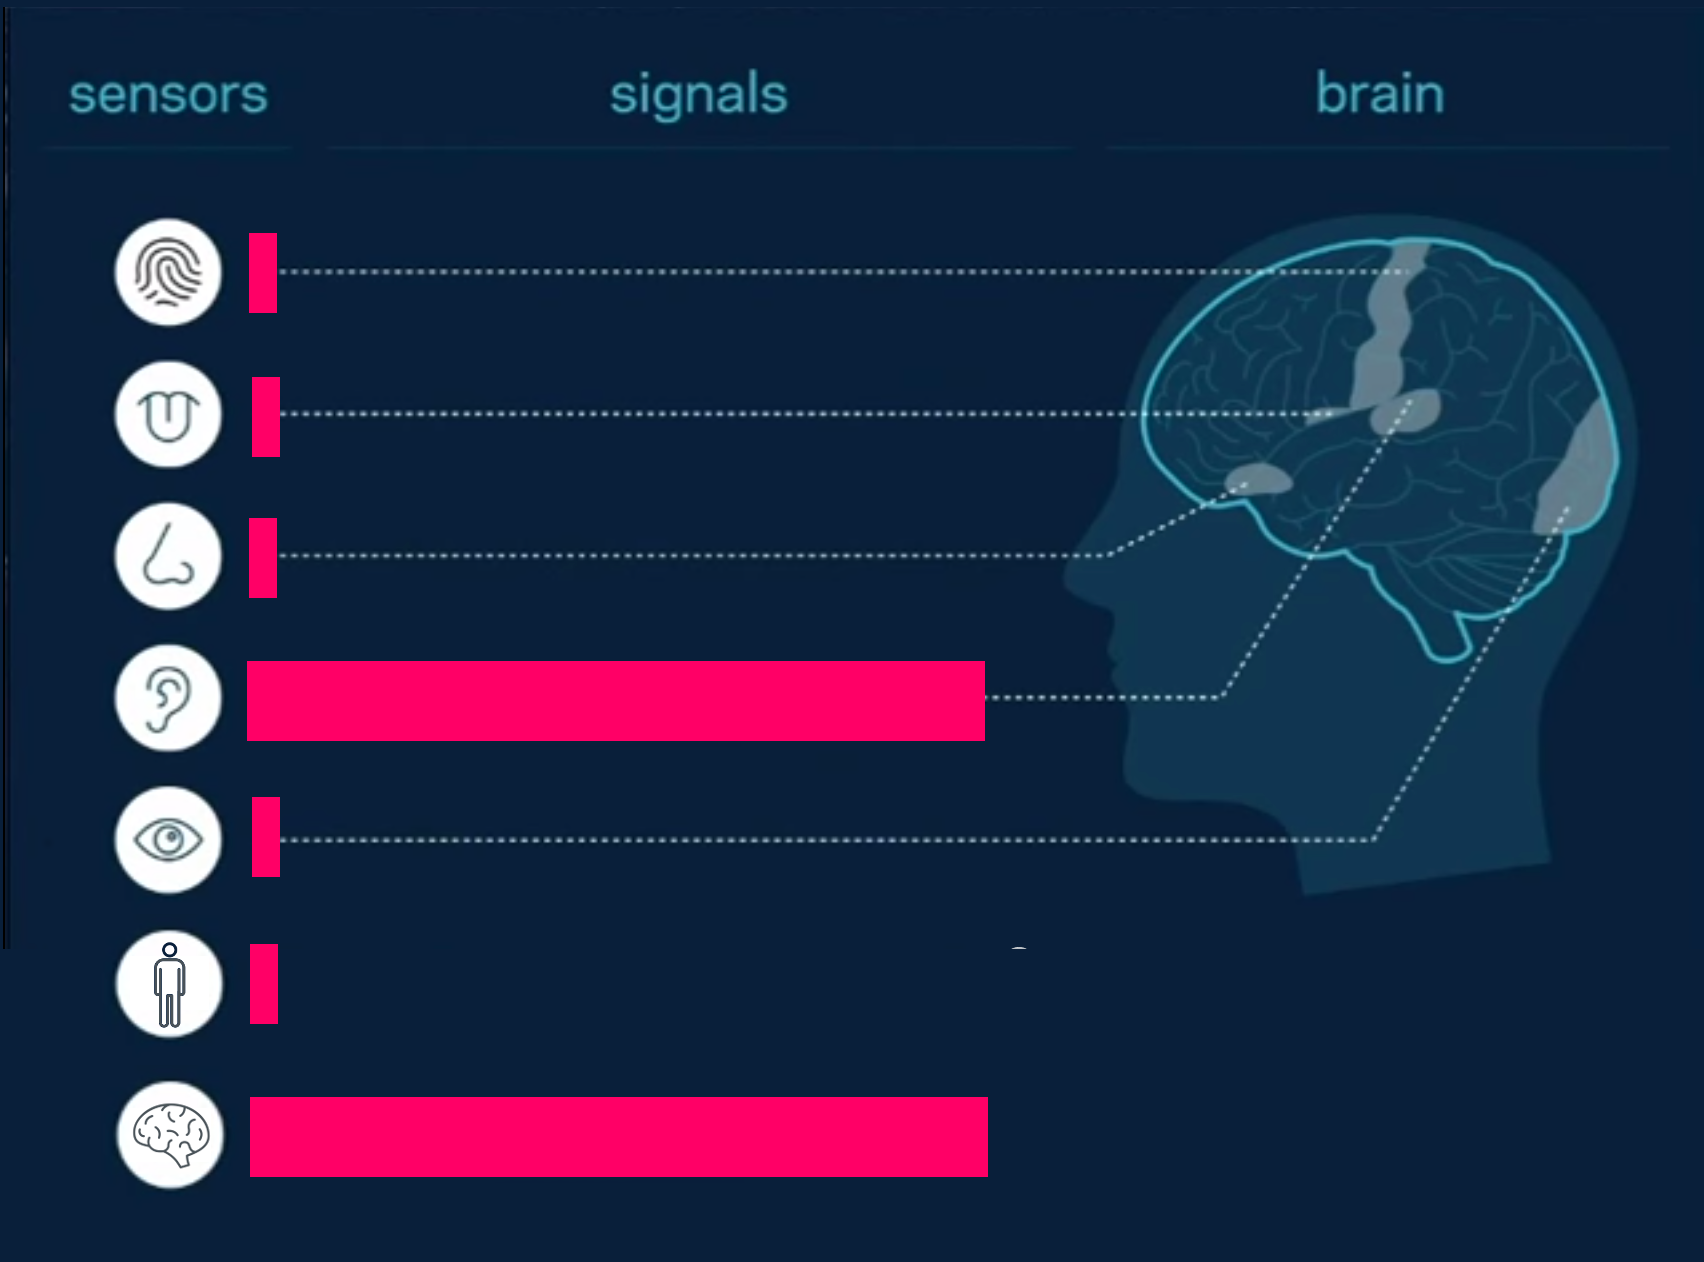
\includegraphics[width=\linewidth]{images/ma-anechoic-chamber.png}
  \end{subfigure}
  \caption{An anechoic chamber and corresponding sense map.}
  \label{fig:anechoic-chamber}
\end{figure}

The map for an anechoic chamber may seem surprising. However, just because the room you are in has a negative decibel rating does not mean you cannot hear. In fact, in this environment, your sense of hearing is likely to be amplified --- and turned inward. You will hear your heart beating, your blood pumping, your digestive system sloshing around. The better the anechoic chamber at swallowing sound, the more intense this experience is going to be.

For this reason, the above anechoic chamber at Orfield Laboratories \cite{orfield} has an unofficial record of 45 minutes for the longest period anyone has sat inside it. As it turns out, hearing one's own bodily functions at deafening internal volumes is likely to cause someone to go a bit crazy, hence the highlighted bar for thought activity.

The above three examples serve as templates with external input guiding one's understanding of what is happening neurologically.


\pagebreak

\begin{center}
  \Huge{Anapana Meditation:}\\
  \Huge{Practicing Focus}
\end{center}

The first 3.5 days of a 10-day Vipassana course are spent practicing ``Anapana'' (breath) meditation. This period is very important as it is time spent practicing acute, one-pointed attention. If we visualize our attention as any skin (internal or external; lips, nose, nostrils, etc.) covered by the pink triangle in Figure~\ref{fig:burmese-anapana-triangle}, we will get an idea of exactly where one's attention is directed at the beginning of Anapana practice.

\begin{figure}[h]
  \centering
  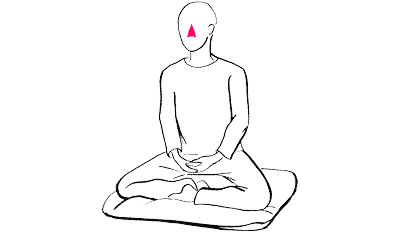
\includegraphics[width=\linewidth]{images/burmese-anapana-triangle.png}
  \caption{Large, triangular Anapana meditation target.}
  \label{fig:burmese-anapana-triangle}
\end{figure}

If you have ever practiced a single-pointed meditation (particularly breath meditations) before, you know all too well how easily your mind can be distracted. Taxes, Mom's birthday, an upcoming meeting, a fun math problem, what's for lunch, the itch on my ear... anything can become a distraction because everything which is not ``my breath'' is by definition a distraction. And we are not accustomed to spending long stretches of time with unwavering, singular focus. We are especially unaccustomed to doing so with all of our attention focused on our breath.

As you practice Anapana for over 30 hours, you will find your attention wandering less and less, while (paradoxically) the distractions become more and more interesting. The itch on your ear becomes an itch on your nose which seems to move with the breath. Your brain will spend less time worrying about taxes and more time trying to solve interesting math problems (if that's your thing).

\begin{figure}[h]
  \centering
  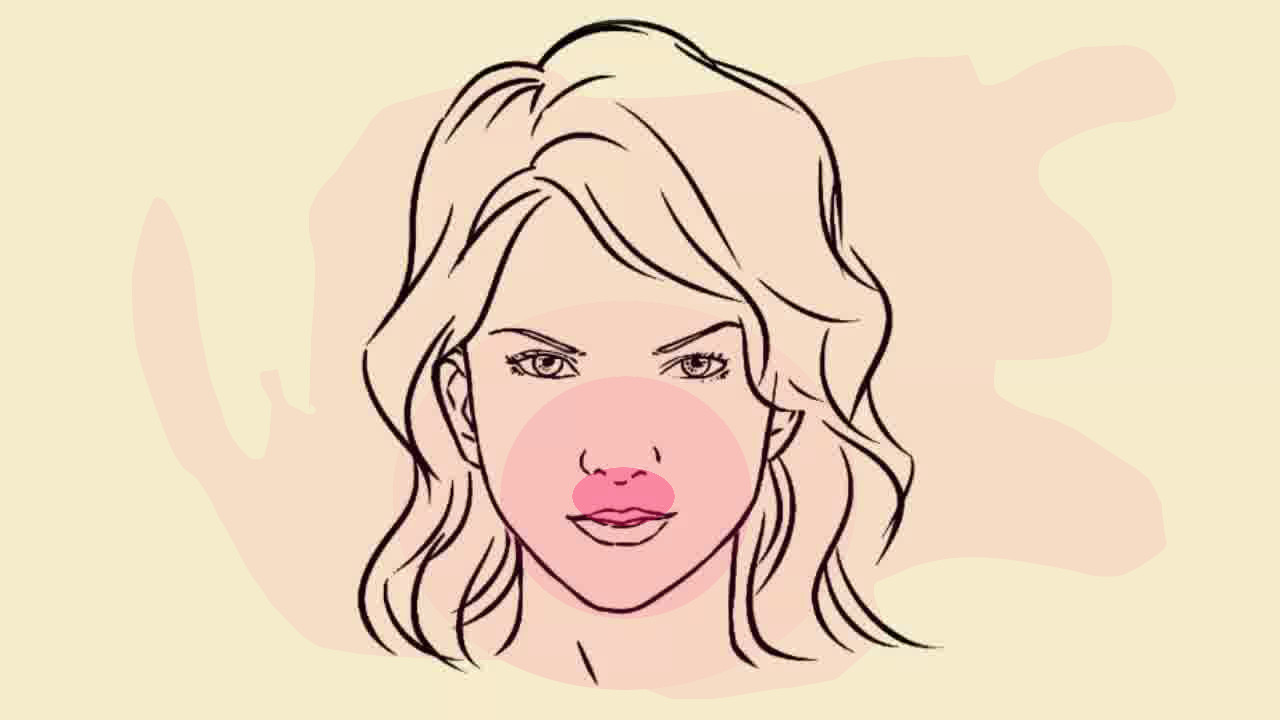
\includegraphics[width=\linewidth]{images/face-attention.jpg}
  \caption{Wandering attention.}
  \label{fig:wandering-attention}
\end{figure}

On the first day, your attention might look something like Figure~\ref{fig:wandering-attention}, where the wavy pink cloud represents any attention spent on any part of the body other than the nostrils or spent ``outside'' the body: on thoughts and emotions. By the fourth day, your attention will often take a shape something like Figure~\ref{fig:narrow-attention}. Over the course of the first three days, the instructions narrow down one's attention from the nose-and-lips triangle from Figure~\ref{fig:burmese-anapana-triangle} to a finger-tip-sized area wherever the breath can be felt beneath the nostrils.

\begin{figure}[H]
  \centering
  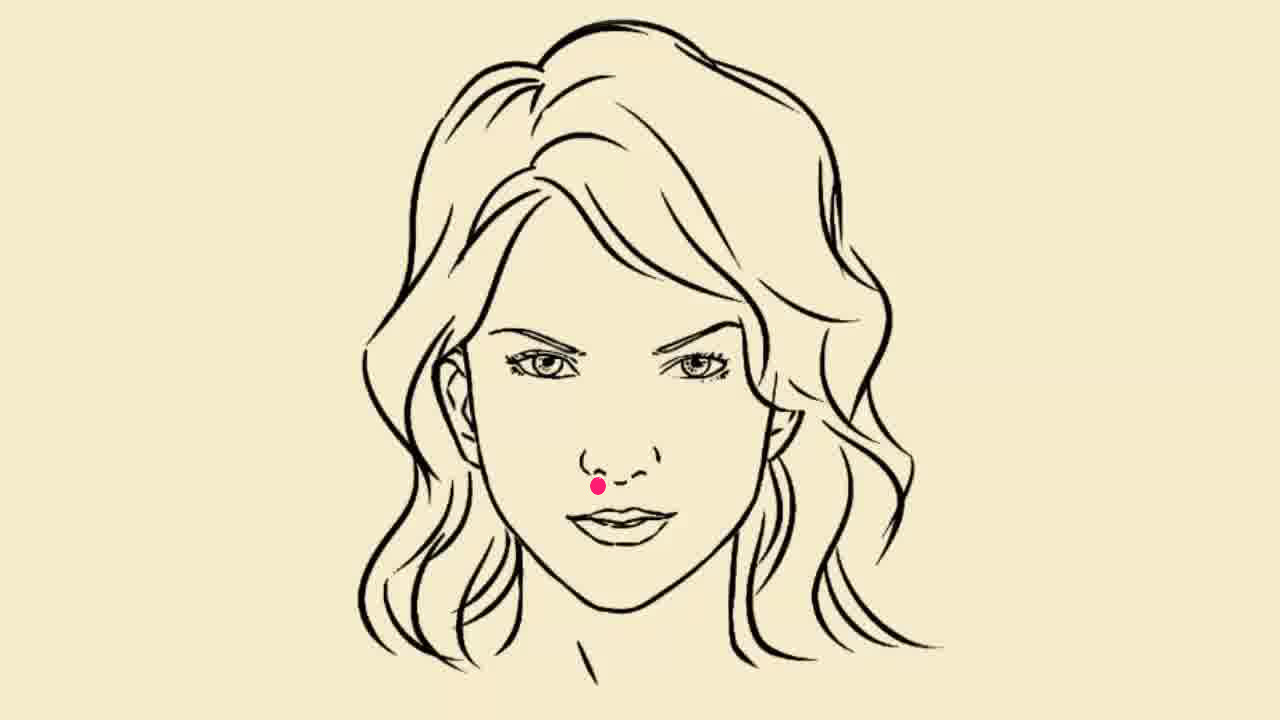
\includegraphics[width=\linewidth]{images/face-attention-narrow.jpg}
  \caption{Narrow attention.}
  \label{fig:narrow-attention}
\end{figure}

If we revisit the notion that ``meditation is a thing'', we can see a specific example in Anapana with the help of the sense map in Figure~\ref{fig:anapana-sense-map}. Where mindfulness and violin, albeit useful physical and mental practices, are not meditation, we can see from the sense map that Anapana \textit{is} meditation. It is the practice of narrowing one's attention, repeatedly, toward a specific sense (in this case, touch) at a specific time (now) in a specific place (just beneath the nostrils). As our skill in Anapana improves, we come nearer and nearer to the focus-oriented meditation ideal of an unwavering single point of awareness.

\begin{figure}[H]
  \centering
  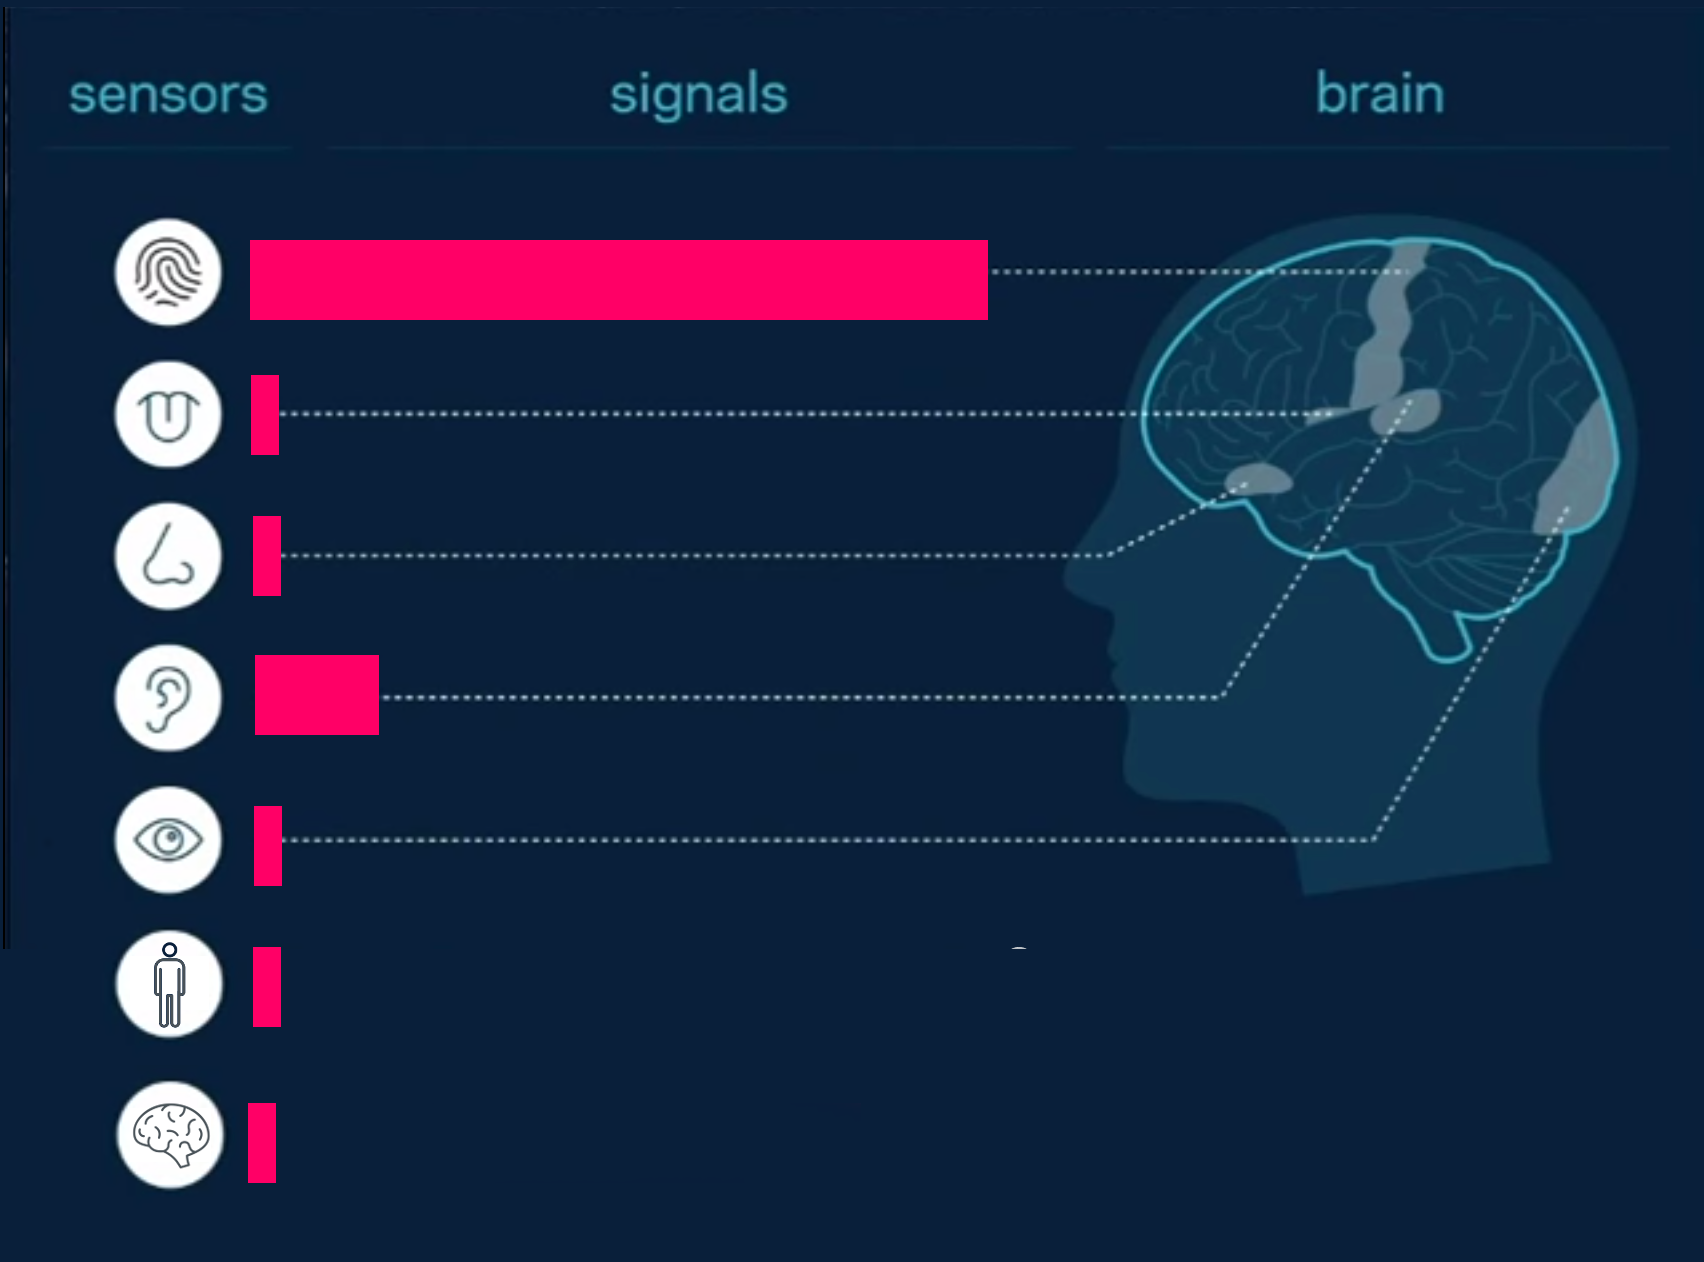
\includegraphics[width=10cm]{images/ma-anapana.png}
  \caption{Anapana sense map.}
  \label{fig:anapana-sense-map}
\end{figure}

In Figure~\ref{fig:anapana-sense-map}, we can see that in reality our attention is not perfectly tuned and narrowed to a tiny spot under our nose. We are still likely to hear sounds around us on the third day of the course, especially if the sound is monkeys clambering over the roof of the meditation hall. By the third day of the course, however, one's attention to sound is likely to be greatly reduced.

For the rest of this paper, make note of the fact that \textit{distraction} is at this stage, and will forever remain, the most important aspect of meditation; it is everything meditation is not, and therefore a significant consideration in all the techniques which follow. Meditation is essentially comprised of only two components: (a) the meditation object and (b) distractions. The activity of meditation is the repeatedly directing of one's attention from the latter to the former.

\pagebreak

\begin{center}
  \LARGE{Anapana: The Bridge}
\end{center}

At the end of the first day of a 10-day Vipassana course, the breath is described as a bridge ``from the known to the unknown, because respiration is one function of the body that can be either conscious or unconscious, intentional or automatic.'' During the 3-day Anapana session of a 10-day course, students are instructed to \textit{consciously} direct attention toward their breath -- and even gently control the breath for brief periods to maintain attention when the mind won't stop wandering -- until awareness of breath, without force, lasts for extended periods. Given that the breath is the one function of the body which operates both consciously and unconsciously, it makes sense that it acts as the starting point for many meditation practices, including Vipassana. The intention of Vipassana is to train the mind out of habits and tendencies which have embedded themselves into the brain and nervous system at an unconscious level. To do this, one must first learn to access one's unconscious. Through the breath, Anapana meditation fulfills this purpose.

Vipassana requires a 10-day course to learn. Anapana does not. Before his death, S.N. Goenka released both 70-minute audio instructions as MP3s for the Anapana meditation technique.\cite{anapana} The 70-minute instructions can be found at \url{http://www.vipassana.co/What-is-Anapana} under ``Anapana Meditation for All'' and come as four 15-minute sessions plus a 10-minute ``daily practice'' session.

\begin{figure}[H]
  \centering
  
\includegraphics[width=8cm]{images/bridge.png}
  \label{fig:bridge}
\end{figure}


\pagebreak

\begin{center}
  \Huge{Vipassana Meditation:}\\
  \Huge{Mutually-Recursive}\\
  \Huge{Consciousness I/O}
\end{center}

Oddly enough, Vipassana mostly seems to be about remaining calm. If you're thinking ``you're sitting there, silent, for 10 hours a day... what is there to get upset about?'' you are in for a surprise. But first, a quick overview of the early mechanics of Vipassana. (See Figure~\ref{fig:vipassana-mechanics}.)
Attention is moved from the nostril area to the top of the head, then systematically moved across every body part, down to the toes. This process then repeats.

This visualization and description is to act as an \textit{example only}: this is not the only way to begin Vipassana meditation. Though Vipassana instruction is systematic, it is far from mechanical or prescriptive. Even in the initial instructions, alternative approaches are offered including alternate orders of observation, alternate areas of observation, and alternate durations of observation. The key aspect of any approach to Vipassana is that the \textbf{entire body} is repeatedly observed within each meditation period.

\begin{figure}[h]
  \centering
  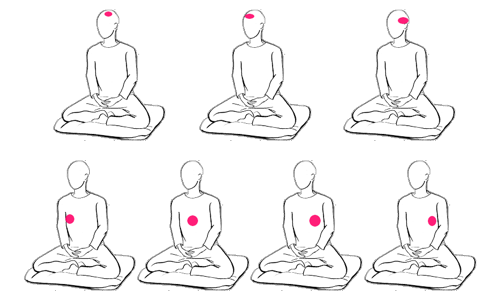
\includegraphics[width=\linewidth]{images/burmese-vipassana-mechanics.png}
  \caption{Simplified example of initial Vipassana mechanics.}
  \label{fig:vipassana-mechanics}
\end{figure}

I will take this opportunity to echo a caveat from the beginning of this paper: This section is in no way a form of instruction. Do not attempt full-body Vipassana meditation outside of a proper 10-day course. Practicing Vipassana is likely the most difficult activity you will ever attempt, should you choose to. To try so alone, you will have no teacher for guidance and the experience is bound to be frustrating.

Consider this warning to also extend to any literature which \textbf{does} attempt to convey Vipassana meditation instruction. Specifically, Glickman's \textit{Beyond the Breath: Extraordinary Mindfulness Through Whole-Body Vipassana Meditation} \cite{glickman} includes a facsimile of instruction provided on a 10-day introductory Vipassana course. Instruction on a course includes 11+ hours of video instruction, at least twice as many hours of audio instruction, and multiple interviews per day with the teacher. Trying to replace this with a book is both inadequate and dangerous.

More complex variations are added to these mechanics as the bodily sensation experienced through this probing of the nervous system becomes increasingly subtle. In this order:

\begin{enumerate}
  \item Add toes-to-head to head-to-toes
  \item Dual/symmetrical observation (both arms, both legs)
  \item Observation of a ``ring'' around the entire body
  \item Observation of as much of the body as possible (while moving attention up and down)
  \item Penetrating attention of muscles, tissues, organs
  \item Penetrating attention of the spinal cord
  \item Randomized attention in fingertip-sized dots throughout the body, inside and out
  \item Sweeping attention through the entire body, up and down, in a single breath
\end{enumerate}

Through this process, attention will move from the sense of touch to all the internal senses and the sense map will look more like Figure~\ref{fig:vipassana-sense-map-1}.

\begin{figure}[H]
  \centering
  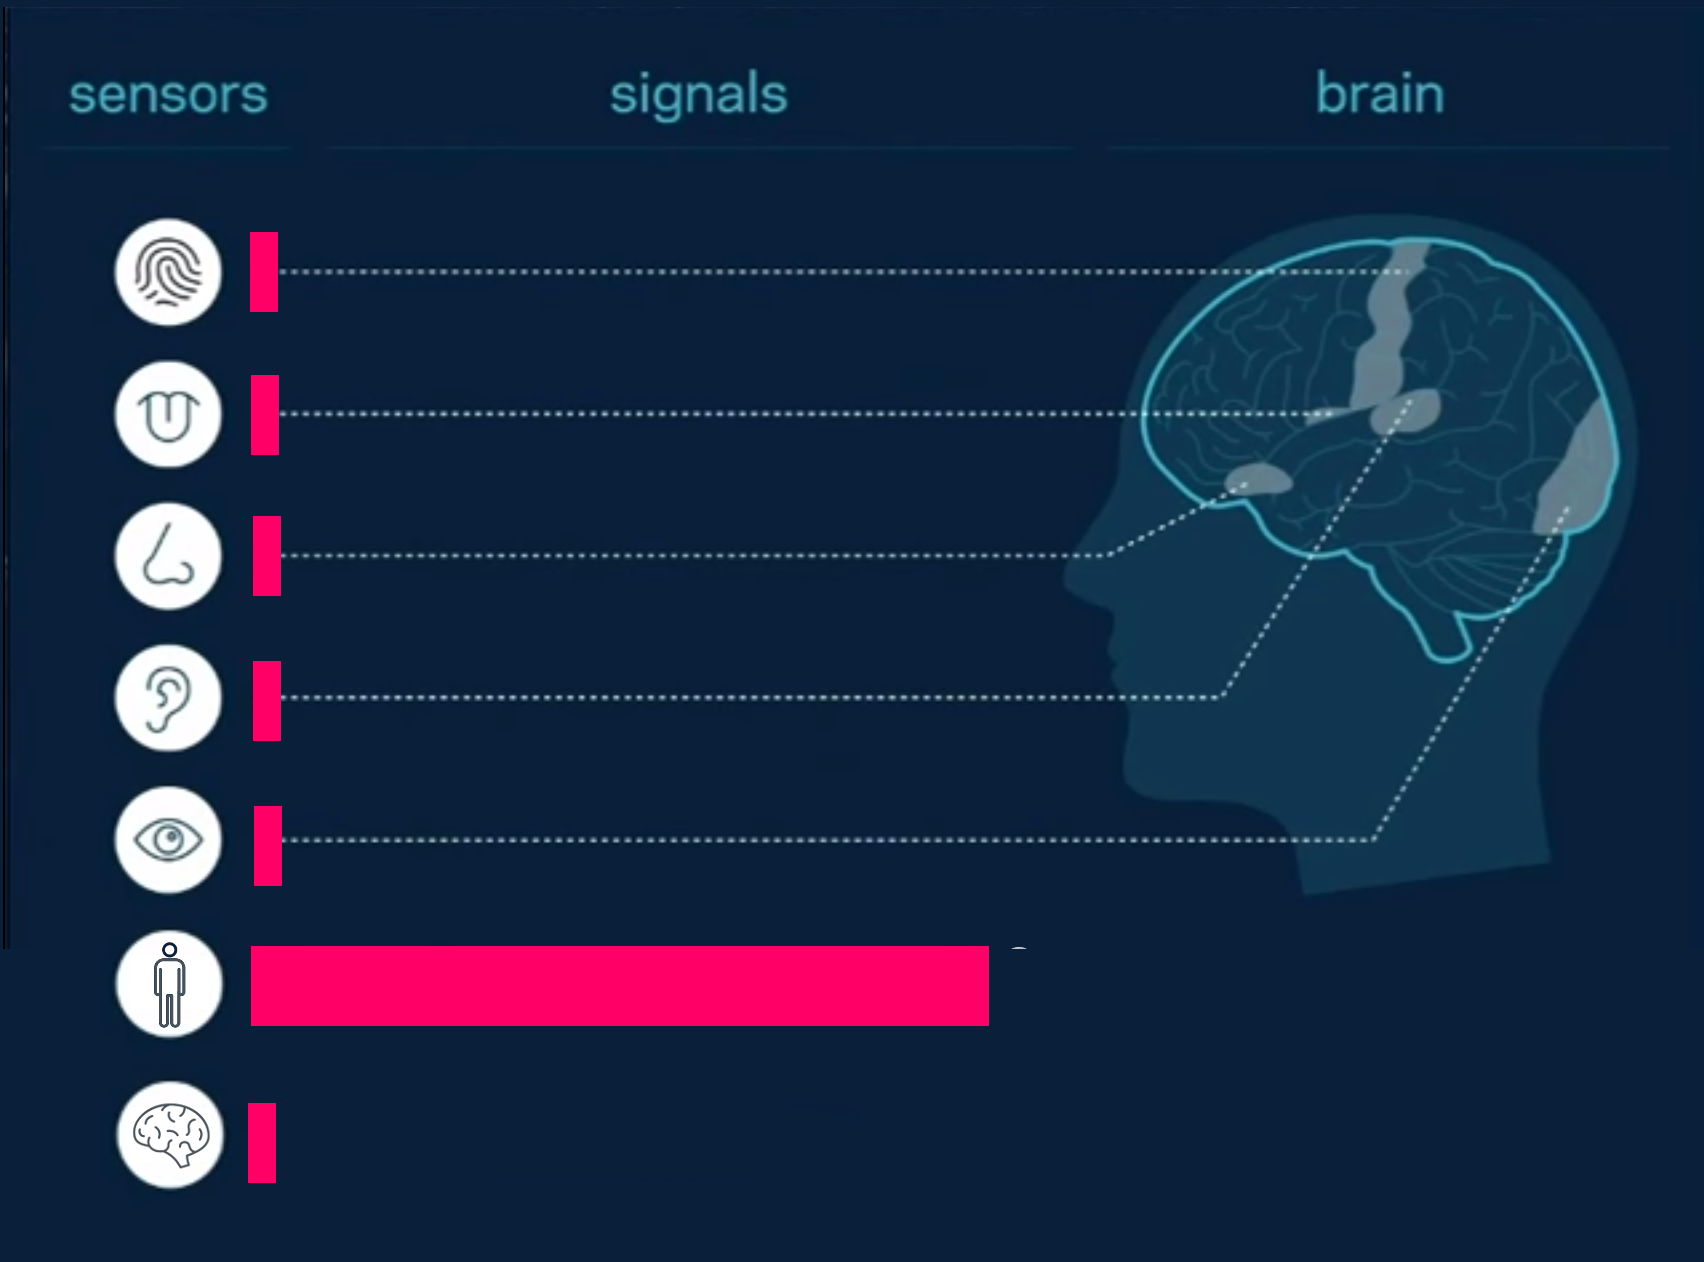
\includegraphics[width=\linewidth]{images/ma-vipassana1.png}
  \caption{Vipassana sense map.}
  \label{fig:vipassana-sense-map-1}
\end{figure}

I should note that I have never successfully penetrated my muscles or inner tissues much. The average new meditator is likely to feel a great many fascinating sensations on her fingertips, palms, arms, toes, and legs. The torso, since it is surrounded in longer nerve fibres, will take longer to observe in the same way. \textit{[citation needed]}

\begin{figure}[h]
  \centering
  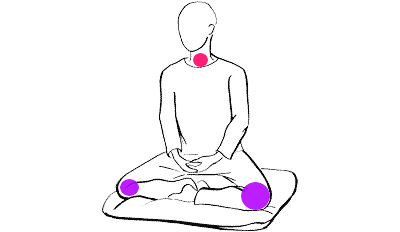
\includegraphics[width=\linewidth]{images/burmese-vipassana-pain.png}
  \caption{Common pain for Westerners in meditative postures.}
  \label{fig:burmese-vipassana-pain}
\end{figure}

As a Canadian who spent little (if any) of my childhood sitting cross-legged on the floor, Figure~\ref{fig:burmese-vipassana-pain} roughly summarizes most of my early meditation experiences, where the purple dots represent intense pain and the pink dot continues to represent my awareness. At the peak of my meditation practice toward the end of a course, I would find that if my attention were somewhere away (say, my neck) from the painful area of my body (say, my knees), I may not feel any pain at all. As I moved my attention around, the pain in my knees would come back as I approached them, but every time I could sustain focus on another part of my body, the pain would appear to decrease with every return visit to my knees. If I can remain calm and focused while away from my knees, my knees' pain seems to take care of itself. If I can remain calm and focused while my attention moves across my knees, the situation continues to improve.

If an individual cannot feel pain in one's knees despite the fact that the pain is ``real'', she has effectively eliminated (some) sensory input. This is possible for all sensory input. The five classic sense-doors will quite clearly shut down in deep meditative states. Just because your eyes are closed does not make you blind. Light sensitivity remains, and as a side bonus of an optic nerve injury from a few years ago, I can ``see'' something (the damaged spot of the nerve) even when my eyes are shut and I'm in complete darkness. This blob which I ``see'' disappears in deep meditative states. Similarly, these deep states of meditation will eliminate audio input as well, which is easier for anyone to detect.


\begin{center}
  \LARGE{Vipassana: The Sledgehammer}
\end{center}

During the Day 4 discourse of a 10-day course, the imagery of the bridge is extended by what is on the far side of that bridge: a giant wall. The wall represents the remaining barrier between the conscious and unconscious mind -- and Vipassana is the tool used to break this barrier. By systematically examining the nervous system, outside-in, one digs through all the layers of unconscious habit as it manifests in bodily sensation.

\begin{figure}[h!]
  \centering
  \begin{subfigure}[b]{0.48\linewidth}
    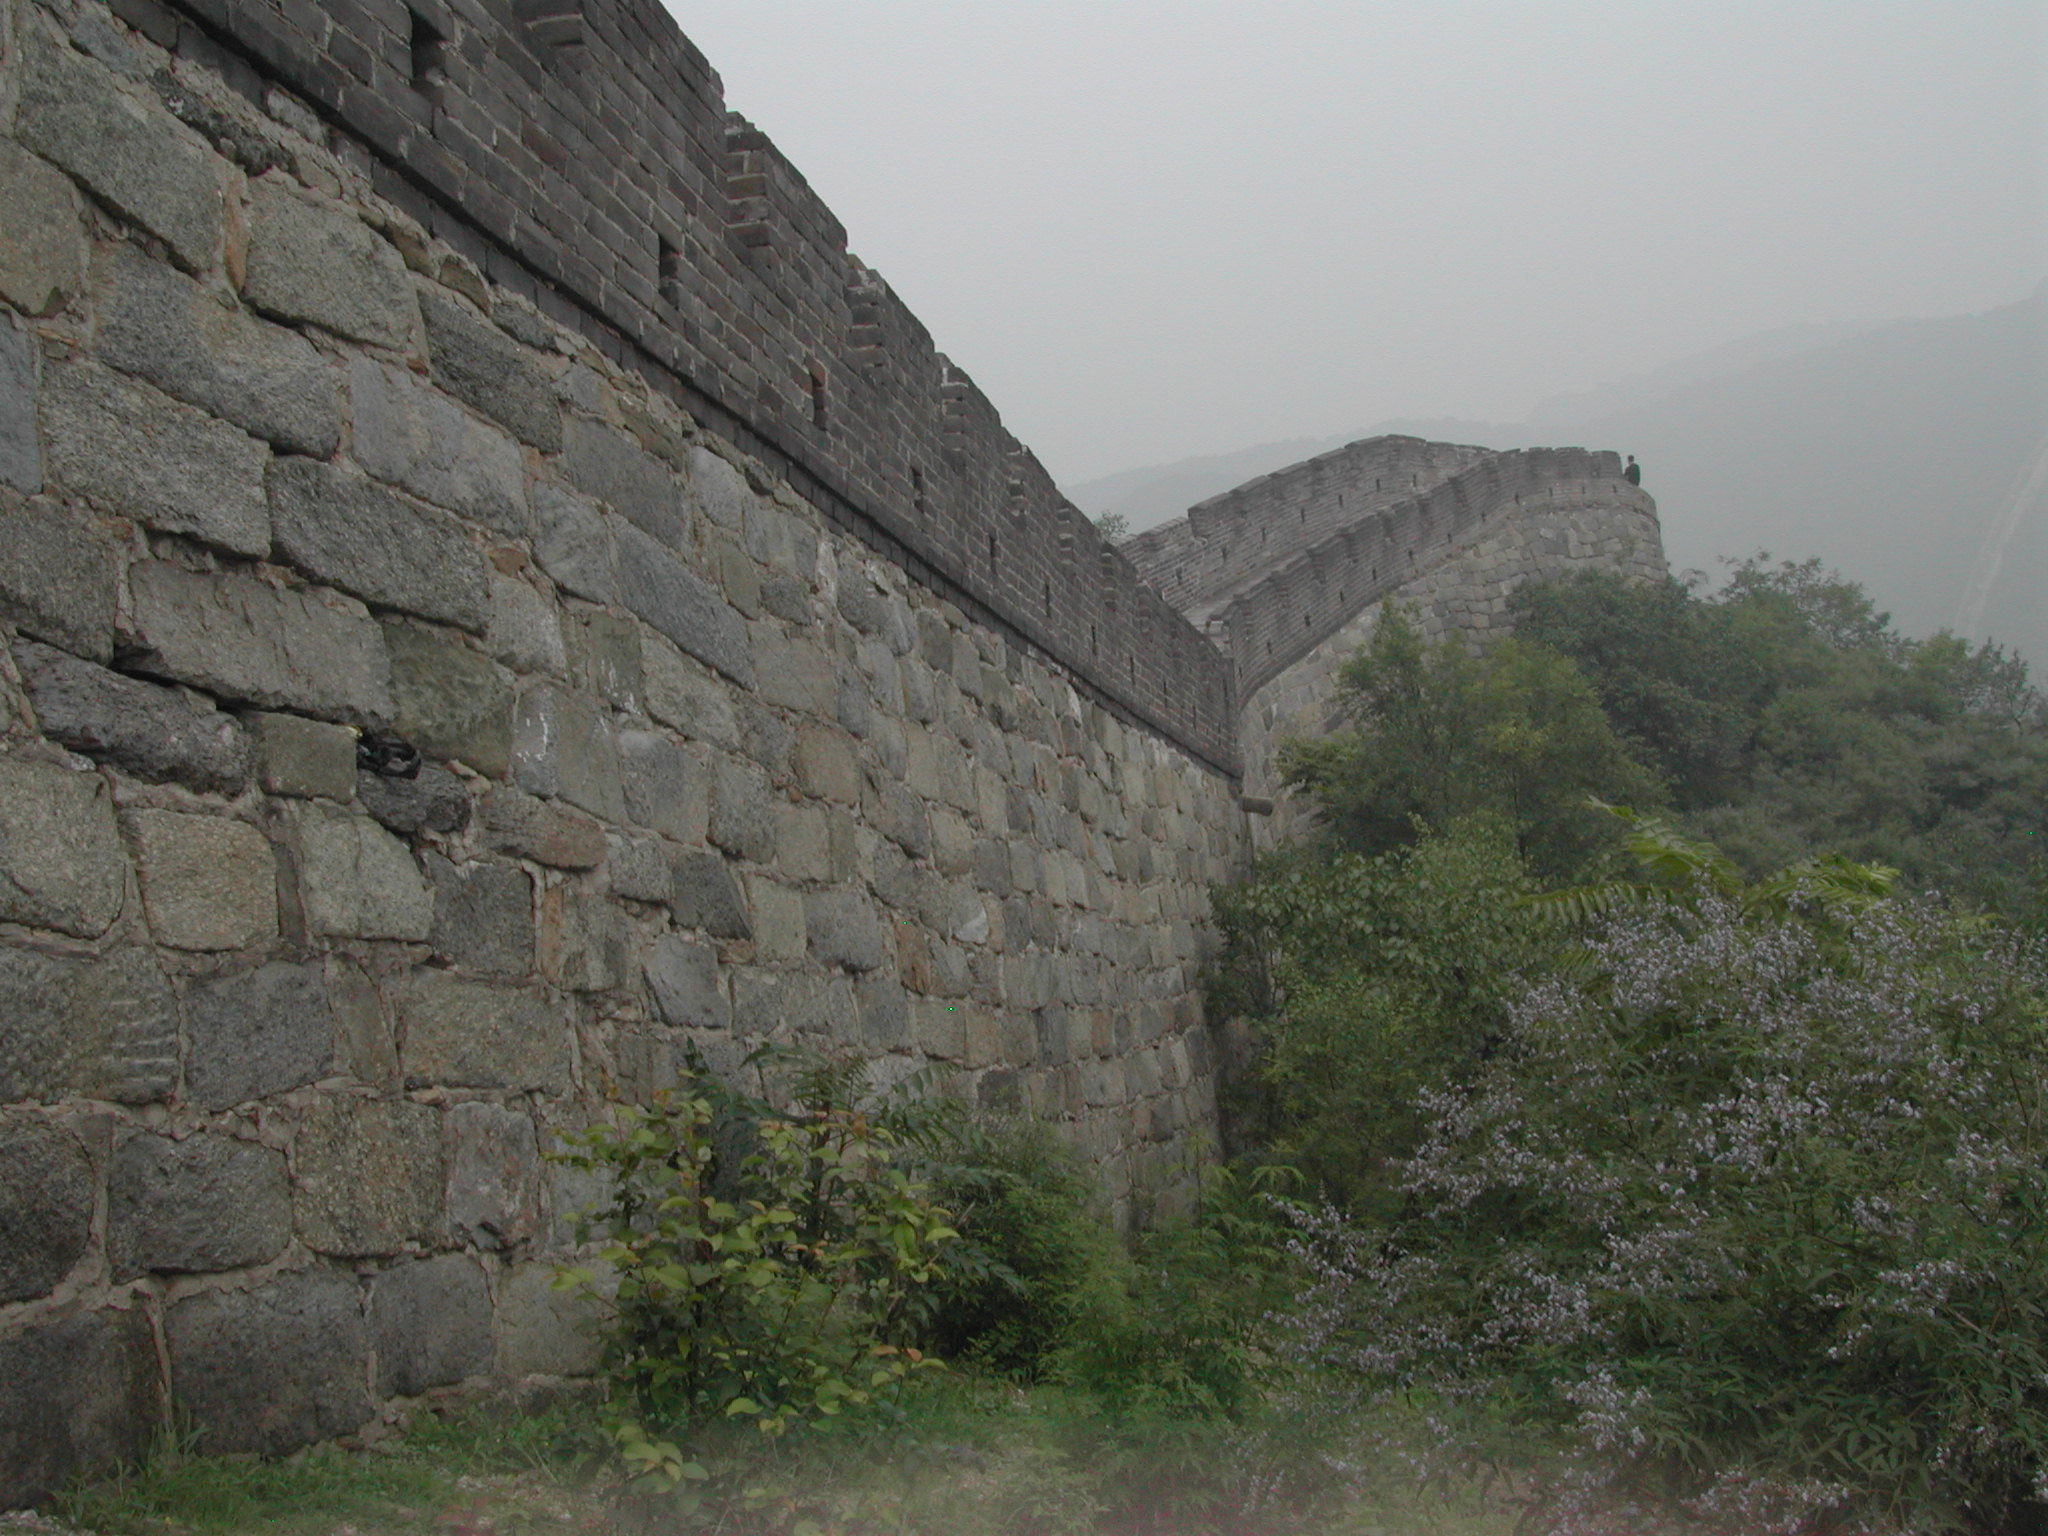
\includegraphics[width=\linewidth]{images/wall.jpg}
  \end{subfigure}
  \begin{subfigure}[b]{0.48\linewidth}
    
\includegraphics[width=\linewidth]{images/bridge.png}
  \end{subfigure}
  \label{fig:wall}
\end{figure}

And what comes of this examination? Sensations in the body are exploded into view and what we normally experience as a narrow band of sensation from the roughly unpleasant to the roughly pleasant: intense sensations like abdominal pain and annoying sensations like uncontrollable itching are gross sensations we normally consider unpleasant; intense sensations like sexual contact and light sensations like touching fur are gross sensations we normally consider pleasant.

This explosion of sensation occurs on an entirely new axis. The range can still be considered pleasant to unpleasant but ``pleasant'' begins to cover new, previously unexperienced territory. These experiences have little or no parallel in mundane life and are best described as ``subtle'': fine oscillations and vibration. This new axis of experience is the sledgehammer used to break through the wall separating conscious from unconscious. Unpleasant sensations and pleasant sensations, both, undergo change. As one observes this change, the change itself comes faster and faster and becomes easier and easier to observe. The goal is to avoid reacting to unpleasant sensations with aversion and to avoid reacting to these newfound pleasant sensations with craving. The task is harder than it sounds. However, the calmer a meditator remains while exploring these new depths, the further she explores.

Unfortunately, unlike Anapana meditation, there is no way to learn Vipassana from an MP3. This practice of observing subtler and subtler sensation requires quite a bit of time, assistance from a live teacher, and repeated instruction. The only way one can learn the technique of Vipassana is to take a 10-day course.


\pagebreak

\begin{center}
  \Huge{Blue Bars:}\\
  \Huge{The New Distractions}
\end{center}

At this point, we can revisit distraction. Distraction is really the essence of meditation. Whether it's taxes, math problems, hunger, itching, or pain... our job as meditators is to accept the presence of a distraction and return our attention to our meditation object.

However, once the pink bars have reduced far enough, once the mind is quiet enough, an entirely new form of distraction emerges. This diagram highlights the first likely candidate for the New Distraction: thought.

\begin{figure}[h]
  \centering
  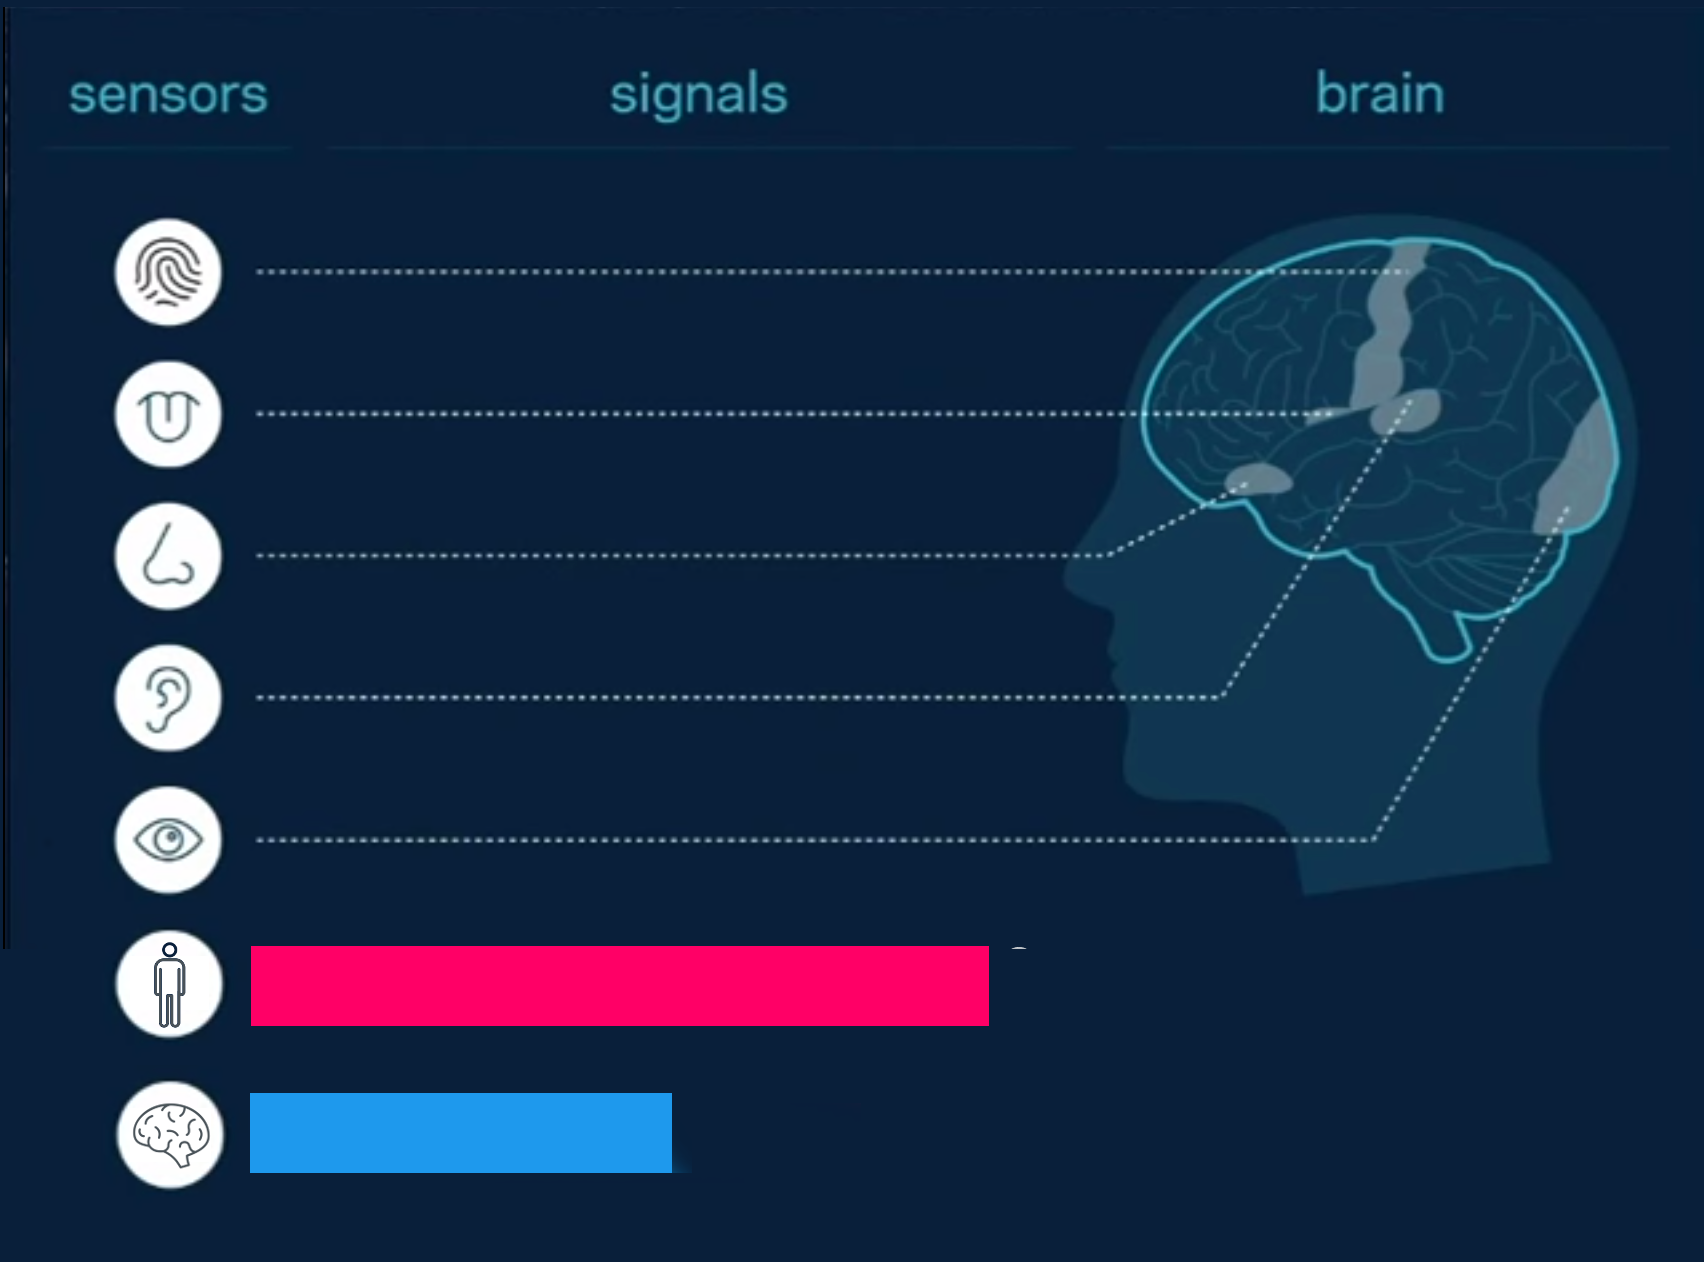
\includegraphics[width=\linewidth]{images/ma-vipassana3.png}
  \caption{Attention on a new distraction.}
  \label{fig:vipassana-sense-map-2}
\end{figure}

These distracting new ``thoughts'' are not normal thoughts in any sense of the word you are currently familiar. These ``thoughts'' are an entirely new form of brain activity caused by your constant prodding of the nervous system through Vipassana. Everything in blue, unfortunately, falls into the ``explaining the concept of `white' to a birth-blind man'' category of unexplainable sensory input. Though this brain activity cannot be explained it \textbf{can} be experienced directly and even a first-time meditator is likely to experience such brain activity on her first 10-day course. The blue bar in Figure~\ref{fig:vipassana-sense-map-2} does not represent a goal or form of meditation, nor even a binary state. Rather, if we imagine brain activity on a continuum, worries about taxes might appear on the far left, interesting math and logic problems in the centre, and the ``blue bars'' of unexplainable thought on the right. However fascinating a journey toward this brain activity may be, the thought processes themselves remain nothing more but a distraction from our goal.

What is meant by ``prodding our nervous system'' and what does this have to do with brain activity? Our second suspension of disbelief was of the deep and intense connection between the brain and the nervous system. We cannot feel the brain directly --- or at all. Thanks to the deep interconnection between the brain and the nervous system, however, the body acts as a surface to which we have ready access --- and which in turn provides us access to the brain. This brain/body connection can be thought of as \textit{mutual recursion}, as the term is used in the previous section.

That the brain/body connection is \textit{mutually recursive} is meant operationally, not existentially. We do not mean to say that the brain could not live without the nervous system (or vice-versa) but that every event --- every operation --- occurring in the nervous system has a corresponding event in the brain, and so forth. This mutually recursive process will eventually wear itself out. If it did not, the advent of slight anger would mean we would, from that moment onward, just get angrier and angrier for the rest of our lives. However, during the process of mutual recursion we can be feeling pain in a knee, to which our emotional response is ``argh, I hate pain'', which makes us angry, which clenches up our physical systems, which makes the pain worse, and so on.

This stack of mutually-recursive operations is what produces all thought, emotion, and sensation. Vipassana is the process of unwinding the stack: If I can pay attention to my aching knee, remain calm and continue to observe it, slowly my body unclenches, the pain subsides a little, my emotional response is calmer, I am able to remain calm longer, and so on.


\pagebreak

\begin{center}
  \Huge{Blue Bars 2:}\\
  \Huge{The New-New Distractions}
\end{center}

Let us quickly revisit our third suspension of disbelief: ``dissolution of the body is a thing.'' Neuroscience tells us some interesting things about the nature of our sense of self and how it relates to our body. From \textit{Where Am I?} \cite{whereami}:

\begin{quote}
  \textbf{The studies reported that people who had once been able-bodied and then became paralyzed felt… less. Less happy than able-bodied people, less sad than able-bodied people. Just less.}
\end{quote}

\begin{quote}
  \textbf{Our \textit{being} is rooted in a body-state. If I were able to remove from your brain, the representation of your body, you would not know that you were you.}
\end{quote}

...which would seem in line with experiences described by mastered meditators of having ``no I'' or ``no self'' as their fundamental insightful discovery. It also seems necessary to project our experiences from one 10-day Vipassana course into the future, with respect to the extent to which this practice can take us. If it were stated that we could explore the entirety of the nervous system and its relationship to the brain --- but not the gallbladder or spinal cord because those are off-limits --- we would have reason to believe that there is a portion of the body and/or nervous system which is exempt from the rules governing these interactions.

Assuming we can explore to the very depths of our nervous system by repeatedly and systematically penetrating it with our attention, given the extent to which this observably occurs on a 10-day course, we can then examine ``mutually-recursive consciousness I/O'' in its totality. What occurs?

\begin{figure}[h]
  \centering
  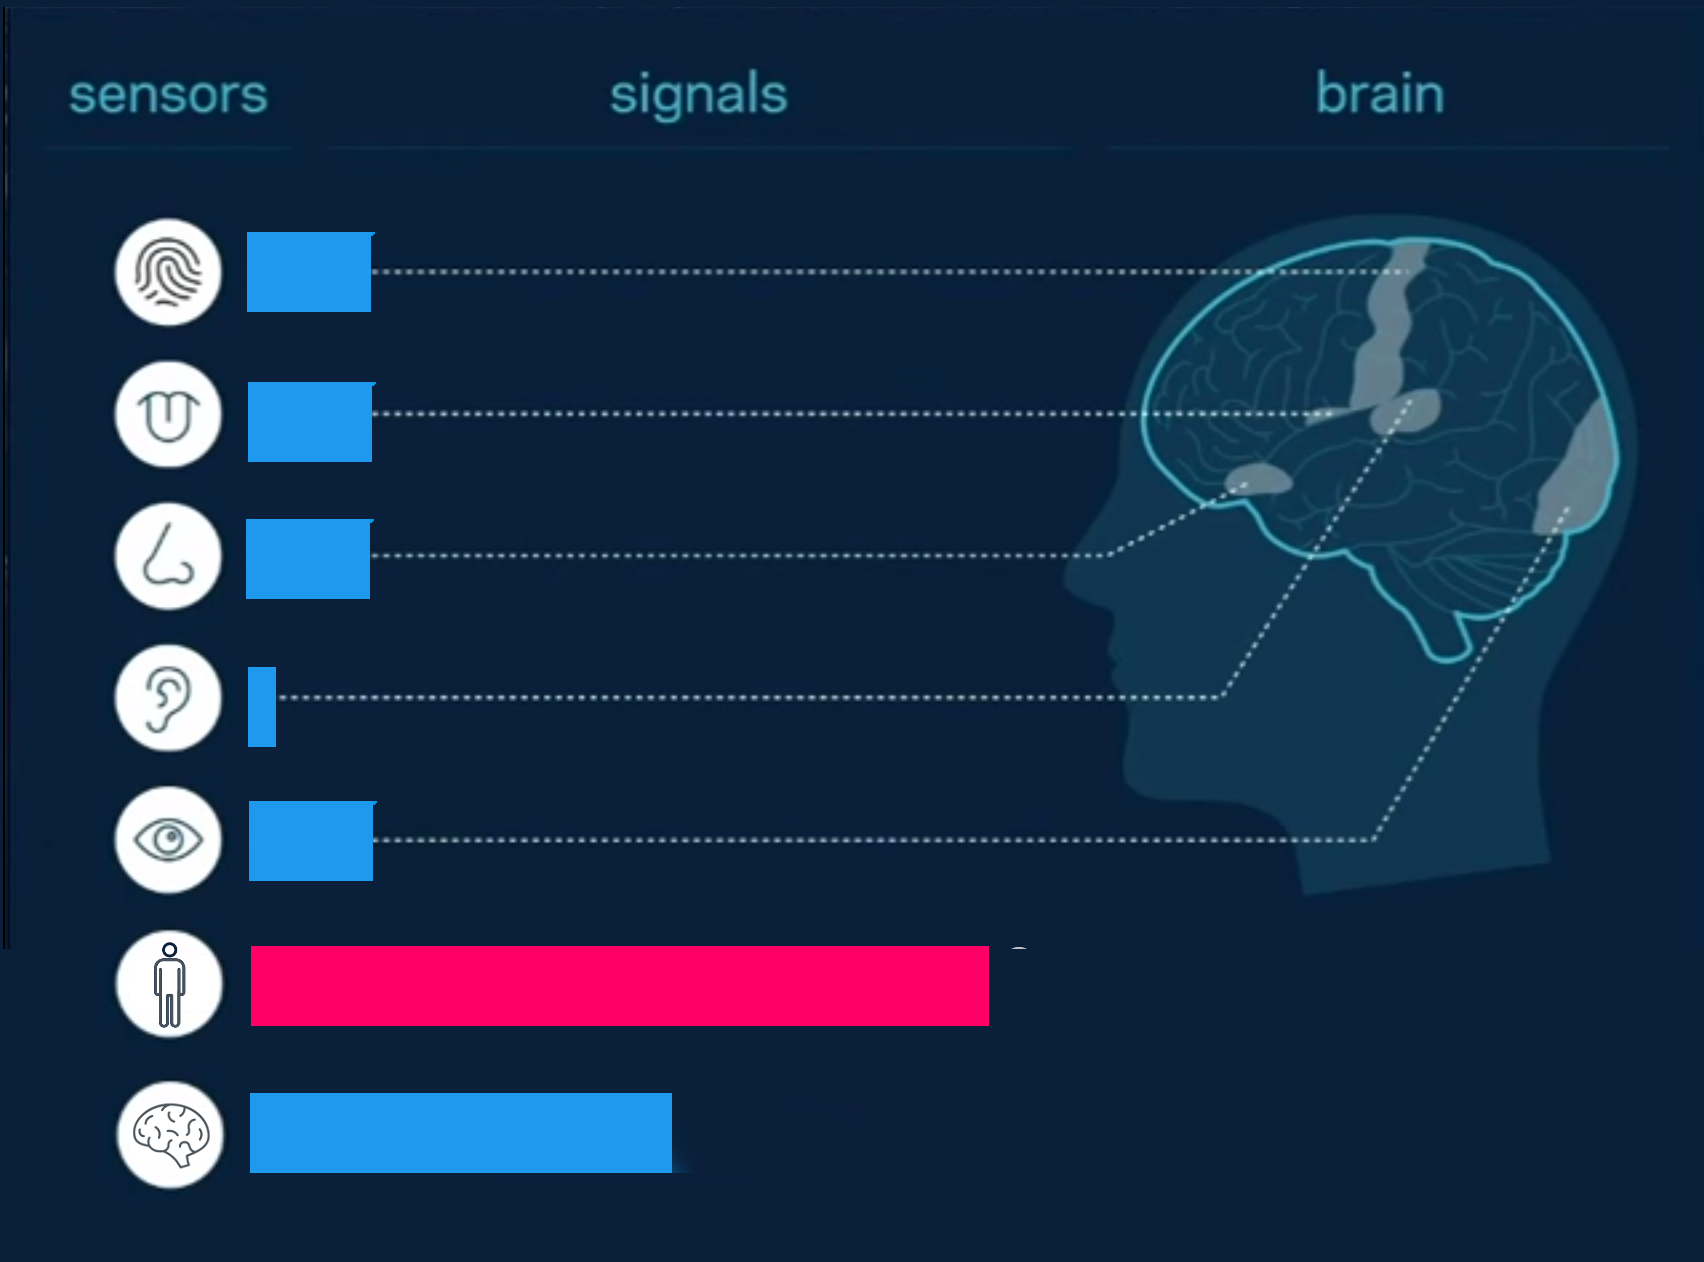
\includegraphics[width=\linewidth]{images/ma-vipassana4.png}
  \caption{Attention distracted by all-new senses.}
  \label{fig:vipassana-sense-map-4}
\end{figure}

This I/O feedback between the brain and body appears to create \textit{a completely new kind of distraction, which goes well beyond new thought patterns}. An attempt to highlight this form of distraction is given in Figure~\ref{fig:vipassana-sense-map-4}.

Here, all of the sense doors which we have quiesced return to life, as did ``thought'' before them. However, this new sensory input (which remains a distraction... just a very sophisticated distraction) is unlike most of regular experience. The nearest approximation I can come up with would be the experience of taking salvia, an awful drug which is legally permitted in most countries because it is simply not that enjoyable. While I do not at all recommend smoking salvia, the Wikipedia article \cite{salvia} is worth a glance, since the description of hallucinogens is approachable for anyone. The two relevant items from the list of ``immediate effects'' are:

\begin{itemize}
  \item Past memories, such as revisiting places from childhood memory
  \item Overlapping realities, such as the perception of being in several locations at once
\end{itemize}

The effects of deep Vipassana meditation are akin to this, in the sense that one may experience, in its entirety, a completely different time or reality. A comparable, sober experience might be that of a car crash: participants often feel time slow down or stop, which is sensory input completely detached from the normal flow of consciousness. That is where similarities end but the comparisons may help provide us with tangible, and therefore approachable, examples.

It is worth reiterating that the purpose of Vipassana is not to experience altered mental states. New thought patterns and new realities are, again, simply distractions from the meditation itself. The meditation remains the systematic observation of the nervous system.


\pagebreak

\begin{center}
  \Huge{Examples}
\end{center}

While I would like to avoid descriptions of personal experiences, a few may help highlight the above description of new and unfamiliar distracted states of mind.

These examples also serve a secondary purpose. If one searches for ``vipassana'' on YouTube, one will find Goenka's instructional videos, critiques from individuals who could not complete their course, TED talks, and experience reports from individuals who did complete their first course. These experience reports (often titled ``My experience...'') tend to confuse these distracting experiences with the meditation itself. Framing a few examples within this paper should help the reader with this differentiation.

\vspace{1cm}
\begin{center}
  \LARGE{The non-example:}\\
  \LARGE{The Resolution to Paradox}
\end{center}

It would seem that one very common effect of Vipassana during deep meditation is to witness the resolution of paradox. A logical, mathematical, or linguistic paradox might emerge in the meditator's mind and just as quickly, it is resolved.

These would appear to mirror Zen koan practice, where the paradox is presented to the meditator verbally, in advance. No such practice occurs in Vipassana. Paradoxes and their solutions appear to be intrinsic to the human makeup, somehow. While the resolution of paradox may be of acute interest to many hackers, indulging in the consideration of a manifest paradox is as much a tangent and distraction to Vipassana as it is to Zazen.

\vspace{1cm}
\begin{center}
  \LARGE{Holding a Baby}
\end{center}

A friend once had a hallucination-like experience, feeling as though she was teleported to her friend's kitchen, holding her friend's 2-year-old while the child cried. The experience was so raw, realistic, and unexpected that she actually opened her eyes and stood up in her meditation cell.

Such distractions are difficult to overcome, since they appear to replace consciousness and reality itself.

\vspace{1cm}
\begin{center}
  \LARGE{Time Slowing Down}
\end{center}

It will become quite clear halfway through a 10-day course that this effect of Vipassana is also quite universal, like paradox and resolution to paradox. The moment-to-moment awareness seems to take longer and longer as the course goes on and each one-hour meditation period can also seem to extend beyond reasonable experiential limit.

However, this is not what I am referring to. The experience of time slowing down in very deep meditative states is that of time slowing down a \textbf{great deal} ...tens or hundreds of thousands of years pass before your awareness in a single meditation period.

It is difficult to describe how this effect remains nothing but a distraction. However, if meditation remains subdivided into two categories, the meditation object and distractions therefrom, we must accept that even experiences which alter our fundamental perceptions are little more than our brain's creative attempts to distract us from the meditation itself.


\pagebreak

\begin{center}
  \Huge{Outcomes}
\end{center}

So, great. Vipassana can trick our bodies and brains to emerge an entirely new set of distractions from the practice of... Vipassana. Why, exactly, would anyone do this?

There is a sketch in \textit{Where Am I?} \cite{whereami} about an arguing couple who must overcome their emotional temptation to get wound up by anger, ending in this wonderful quote:

\begin{quote}
  \textbf{Honey, don’t forget what the half-life is on the autonomic nervous system.}
\end{quote}

The autonomic nervous system is what causes the ``winding stack'' of thought and emotion described earlier. The autonomic nervous system is what makes (and keeps) you angry. And afraid. And sad. And anxious. And everything else you feel.

Vipassana is a systematic practice to calm the nervous system (and brain?) so that every sensory input can be analyzed rationally. You won't become a perfectly rational machine after one 10-day Vipassana course, but you are likely to come out with a much clearer head and a much better capacity for decision-making in general.

I would describe the positive effects of nervous system meditations to live on a spectrum. On one end of the spectrum are the positive, rationality-enhancing qualities of calming one's nervous system with quiet attention. On the other end of the spectrum are the subtler qualities: Meditation seems to make a person more generous, more compassionate, more empathetic. Why would systematic analysis of the autonomic nervous system have these effects? A wide body of research suggests that many forms of meditation, including Vipassana, exhibit these positive effects. Many often identify specifically enhanced activity in the prefrontal cortex \cite{differentialengagement, meditationbrainstructure}, which is identified as the centre of the will to live and altruistic tendencies in the human brain.\cite{personalityneuroscience} However, literature explaining why or how such effects may occur is limited.

Regardless of the mechanism, I do find the entire endeavour not just fascinating, but endlessly worthwhile. Vipassana is simultaneously the hardest thing I have ever done --- and the most valuable.


\pagebreak

\begin{center}
  \Huge{Further Reading}
\end{center}

\vspace{1cm}

\begin{itemize}
\item \textit{The Art of Living: Vipassana Meditation As Taught by S. N. Goenka} (Hart, 1987)
\item \textit{An Atheist's Glimpse of God}, my write-up of my first 10-Day Vipassana course:
  \begin{itemize}
  \item \href{http://blog.deobald.ca/2013/02/an-atheists-glimpse-of-god.html}
             {\nolinkurl{http://blog.deobald.ca/2013/02/}}\\
        \href{http://blog.deobald.ca/2013/02/an-atheists-glimpse-of-god.html}
             {\nolinkurl{an-atheists-glimpse-of-god.html}}
  \end{itemize}
\item \textit{Drugs, meditation, warnings}, my comparison of meditation techniques and various drugs:
  \begin{itemize}
  \item \href{http://blog.deobald.ca/2015/01/drugs-meditation-warnings.html}
             {\nolinkurl{http://blog.deobald.ca/2015/01/}}\\
        \href{http://blog.deobald.ca/2015/01/drugs-meditation-warnings.html}
             {\nolinkurl{drugs-meditation-warnings.html}}
  \end{itemize}
\end{itemize}

\pagebreak

\begin{center}
  \Huge{Appendix A:}\\
  \Huge{Can we ``hack'' Vipassana?}
\end{center}

If Vipassana is hacking the mind, is there an opportunity for hacking Vipassana? Can we hack the hacking process? Let's ask Martin Thompson. The following slide in Figure~\ref{fig:load-test} is from his 2013 talk \textit{Performance Testing Java Applications} \cite{testingjava} and while I have no intention of ostracizing non-computer hackers, software was my career once upon a time and the example is not only appropriate but reasonably accessible.

\begin{figure}[h]
  \centering
  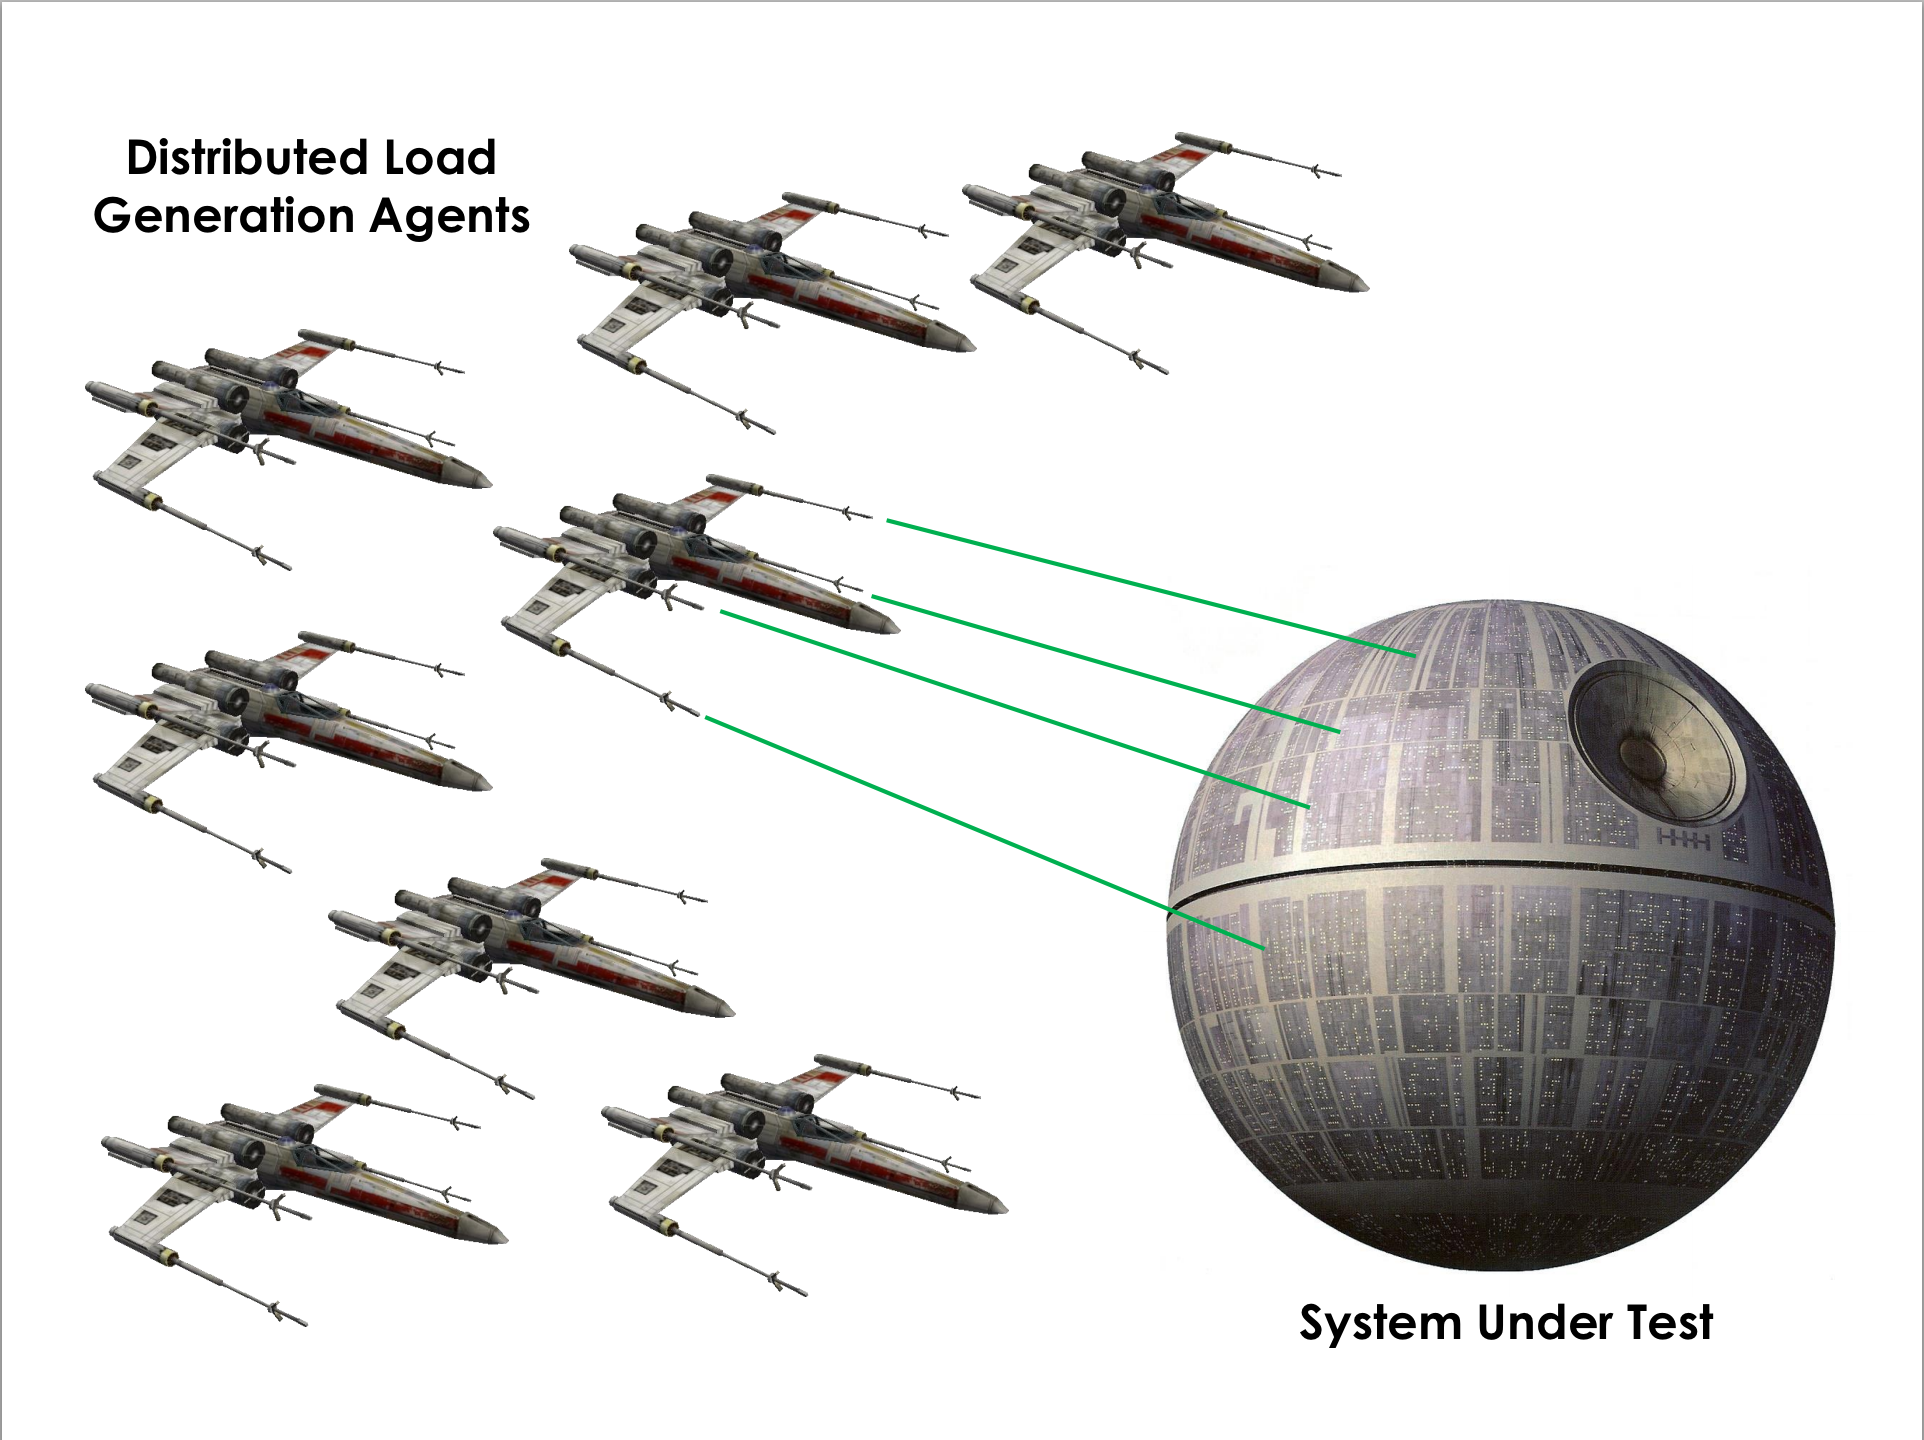
\includegraphics[width=\linewidth]{images/deathstar1.png}
  \caption{A computer system under load test.}
  \label{fig:load-test}
\end{figure}

He suggests that any system we intend to observe should be observed through a 3rd party observer by dumping network traffic (see Figure~\ref{fig:objective-load-test}). For computer systems, this makes a great deal of sense. Were the system under test or the load agents (the Death Star and X-Wings, respectively) to perform the measurements, the measurements and the systems would likely interfere with each other.

\begin{figure}[h]
  \centering
  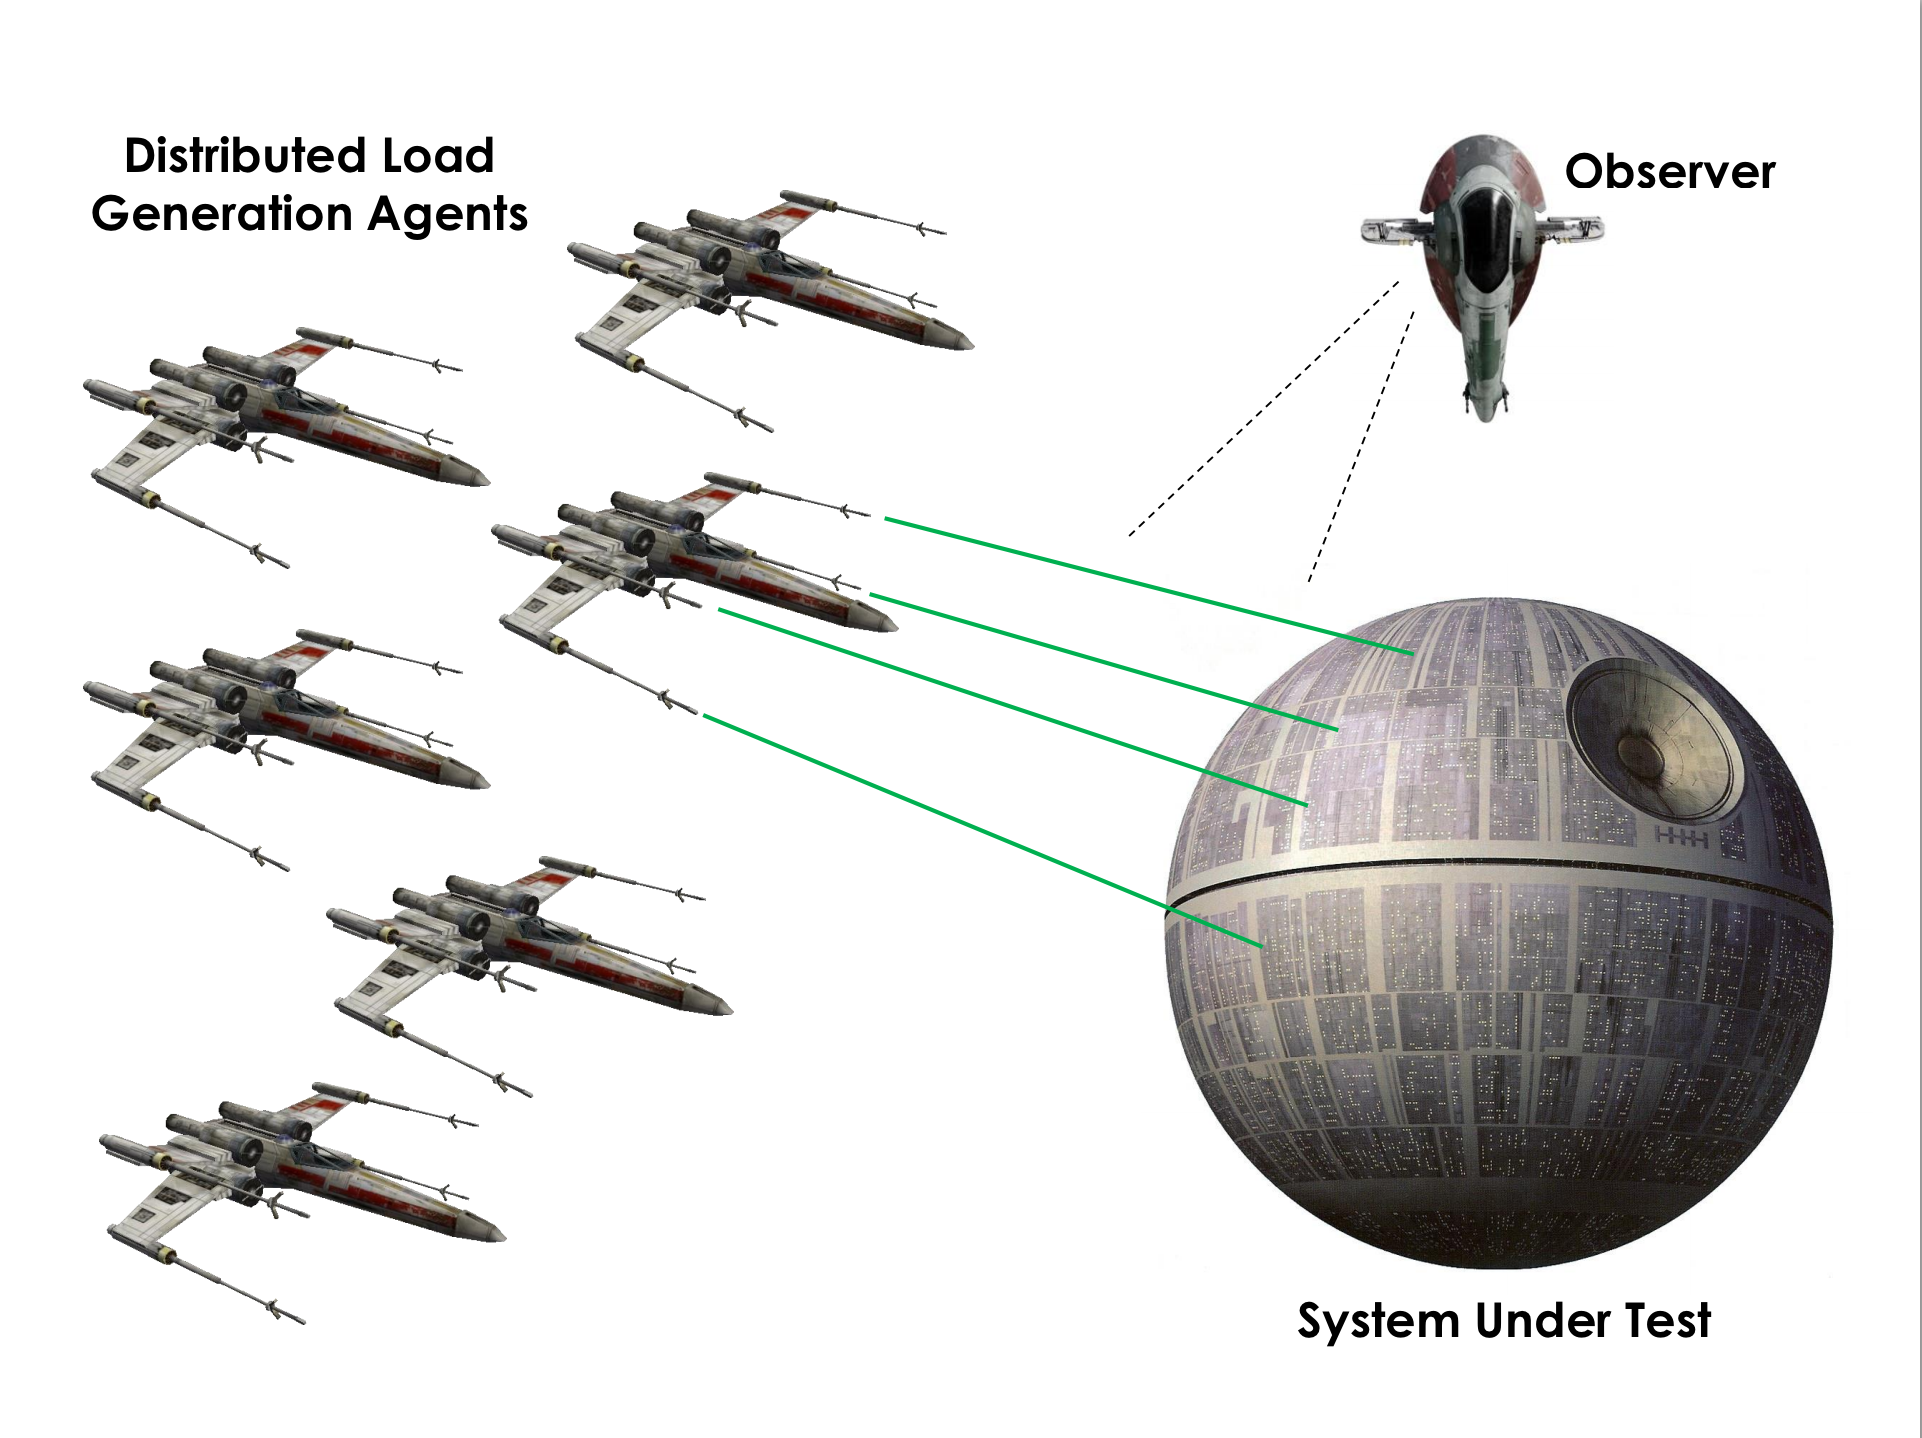
\includegraphics[width=\linewidth]{images/deathstar2.png}
  \caption{A load test with an objective, 3rd-party observer.}
  \label{fig:objective-load-test}
\end{figure}

Unfortunately, human biology is not so keen on this setup. Even if we had the technology to tap into the interactions of the brain and nervous system (we don't), there is no way to observe the interactions of the brain and nervous system without immediately falling into the Matrix Paradox (see Figure~\ref{fig:nervous-system-observer}). How do I know the tool I used is trustworthy? How do I know the observations I made with my eyes are trustworthy? This is all once again external.

\begin{figure}[h]
  \centering
  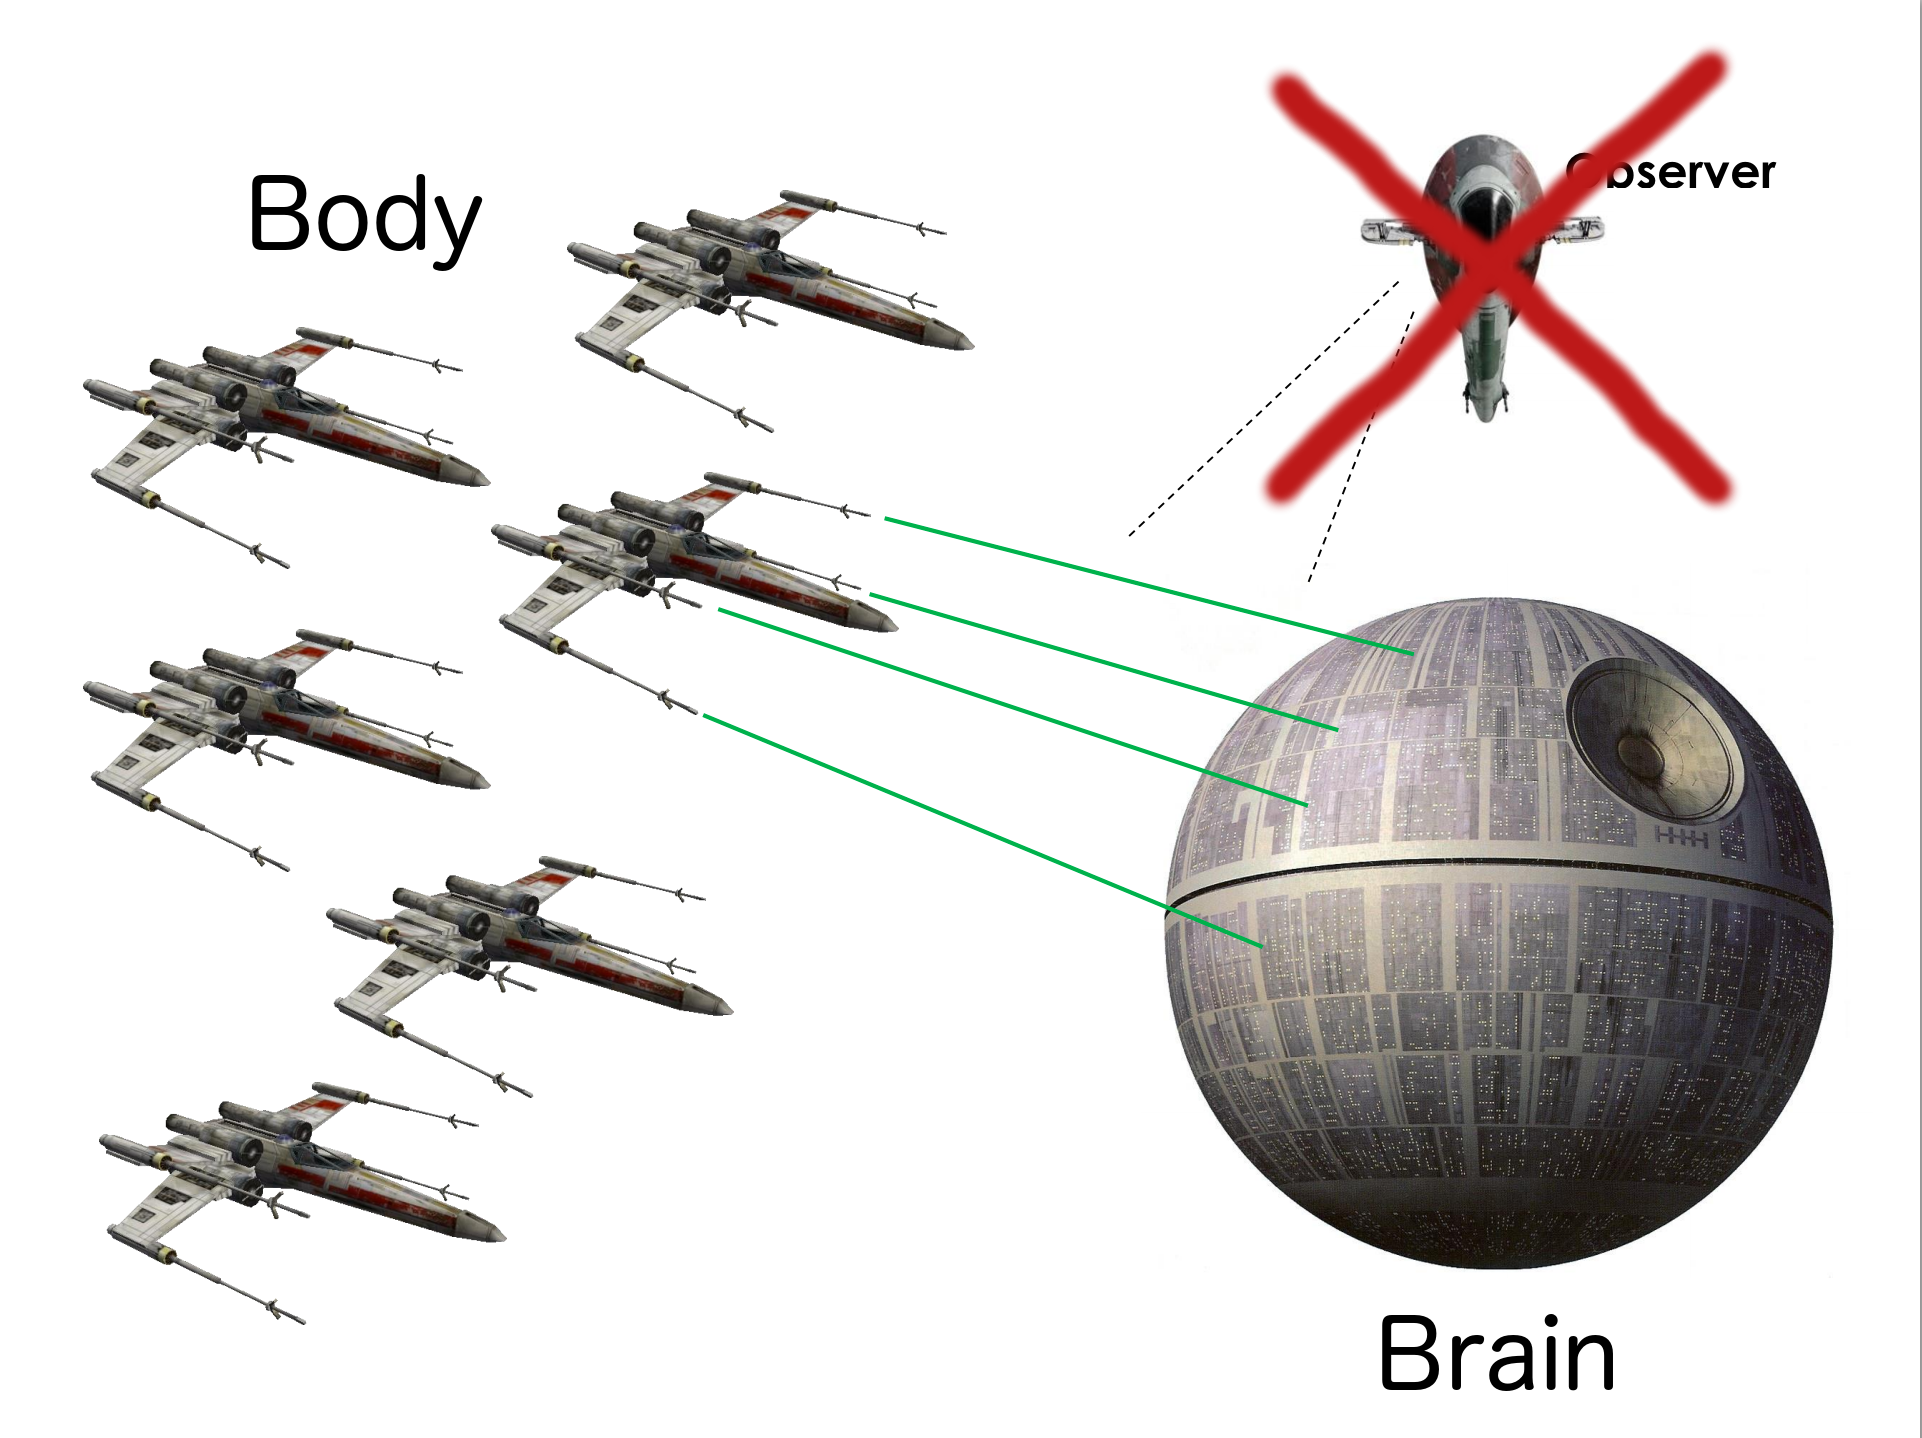
\includegraphics[width=\linewidth]{images/deathstar3.png}
  \caption{The nervous system cannot have an objective observer.}
  \label{fig:nervous-system-observer}
\end{figure}

It is possible to ``jump out'' of Vipassana momentarily to take stock of the effects of the meditation. Did my hearing just cut out? Did I just force my brain to become consciously aware of my normally-unconscious proprioception pertaining to my right arm? Did I just feel my cardiovascular system in exquisite detail or did I imagine it? ...but it is not possible to do so without breaking the meditation for the period of this observation.

I performed this exercise a great deal toward the end of my second 10-day course because I was quite confused about everything that I was experiencing. It framed my understanding but it did little for the practice itself. I don't recommend doing this. Particularly for your first course, try your hardest to follow the instructions precisely and give all of your energy to the moment-to-moment attention demanded of you. Otherwise you will find yourself spending 10 days thinking about meditation, rather than meditating.
Observation of the process itself, rather than observation of your mind via your nervous system, is actually just another clever form of distraction. Every distraction you indulge will limit the positive effects of the meditation.

This particular distraction may feel justified as the reification of your skepticism. While it pays to be skeptical, try your hardest to avoid skepticism during the course. Approach the practice skeptically until you decide to take a course and then save your analysis of whatever newfound skepticism the course generates for you until after the course is completed. There will be plenty of time to discuss the meditation and the outcomes of the meditation on the tenth day when talking is permitted; explore your skepticism here. Other meditators are likely to be the only ones who will quite comprehend the concepts you are trying to discuss.

\pagebreak

\begin{thebibliography}{9}
\raggedright

\bibitem{thenewsroom}
  Aaron Sorkin.
  \url{https://www.youtube.com/watch?v=2C6h-Yyx9Yk}
  \textit{The Newsroom}.
  HBO, 2012.

\bibitem{fiveprecepts}
  Edited by Access to Insight.
  \url{https://www.accesstoinsight.org/ptf/dhamma/sila/pancasila.html}
  \textit{The Five Precepts: pañca-sila}
  Access to Insight (BCBS Edition), 30 November 2013.

\bibitem{experiencethetruth}
  S.N. Goenka.
  \url{https://www.youtube.com/watch?v=mcbGbN8pFyk&list=PLlb2aTuor6J9j8hACeX6GUmd4WF7QJsbu&index=2}
  \textit{Experience the Truth}.
  Vipassana Research Institute, 1992.

\bibitem{taocp}
  Donald Knuth.
  \textit{The Art of Computer Programming}.
  Addison-Wesley, 1962, 1968, 1969, 1973, 2005, 2011, 2015, 2017.
  ISBN: 0-201-03801-3

\bibitem{joyofcooking}
  Irma S. Rombauer, Marion Rombauer Becker.
  \textit{The Joy of Cooking, Sixth Edition}.
  Bobbs-Merrill, 1975.
  ISBN: 0-02-604570-2

\bibitem{hackerhowto}
  Eric S. Raymond: How To Become A Hacker,
  \url{http://www.catb.org/esr/faqs/hacker-howto.html}

\bibitem{abrashvr}
  Michael Abrash.
  \url{https://www.youtube.com/watch?v=UDu-cnXI8E8}
  \textit{Why Virtual Reality Will Matter to You}.
  Facebook F8 Summit, Fort Mason, 2015.

\bibitem{simulationhypothesis}
  \url{https://en.wikipedia.org/wiki/Simulation_hypothesis}
  \textit{Simulation Hypothesis}.
  Wikipedia.

\bibitem{ramachandranbrainfunction}
  V. S. Ramachandran, Eric L. Altschuler.
  \url{https://academic.oup.com/brain/article/132/7/1693/328686}
  \textit{The use of visual feedback in restoring brain function}.
  Brain, 132(7):1693–1710, July 2009.

\bibitem{proprioception}
  \url{https://en.wikipedia.org/wiki/Proprioception}
  \textit{Proprioception}.
  Wikipedia.

\bibitem{nocioception}
  \url{https://en.wikipedia.org/wiki/Nociception}
  \textit{Nocioception}.
  Wikipedia.

\bibitem{fmrihunger}
  Dagmar Führer, Stefan Zysset, Michael Stumvoll.
  \url{https://www.ncbi.nlm.nih.gov/pubmed/18292747}
  \textit{Brain activity in hunger and satiety: an exploratory visually stimulated fMRI study}
  Obesity, 16(5):945-50, May 2008.

\bibitem{whereami}
  Jad Abumrad, Robert Krulwich.
  \url{http://www.radiolab.org/story/91524-where-am-i/}
  \textit{Where Am I?}
  RadioLab, May 2006.

\bibitem{orfield}
  Lindsey Galloway.
  \url{http://www.bbc.com/travel/story/20121022-the-quietest-place-on-earth}
  \textit{The quietest place on Earth}
  BBC, 23 October 2012.

\bibitem{anapana}
  S.N. Goenka
  \url{http://www.vipassana.co/What-is-Anapana}
  \textit{What is Anapana?}
  Vipassana Research Institute, 21 October 2016.

\bibitem{glickman}
  Marshall Glickman.
  \textit{Beyond the Breath: Extraordinary Mindfulness Through Whole-Body Vipassana Meditation}.
  Tuttle Publishing, 2002.
  ISBN: 1582900434

\bibitem{salvia}
  \url{https://en.wikipedia.org/wiki/Salvia_divinorum}
  \textit{Salvia divinorum}.
  Wikipedia.

\bibitem{differentialengagement}
  Holzel B.K., Ott U., Hempel H., Hackl A., Wolf K., Stark R., Vaitl D.
  \textit{Differential engagement of anterior cingulate and adjacent medial frontal cortex in adept meditators and non-meditators}
  Neuroscience Letters, 421:16–21, 2007.

\bibitem{meditationbrainstructure}
  Fox, Kieran C.R.; Nijeboer, Savannah; Dixon, Matthew L.; Floman, James L.; Ellamil, Melissa; Rumak, Samuel P.; Sedlmeier, Peter; Christoff, Kalina
  \textit{Is meditation associated with altered brain structure? A systematic review and meta-analysis of morphometric neuroimaging in meditation practitioners}
  Neuroscience \& Biobehavioral Reviews, 43:48–73, June 2014.

\bibitem{personalityneuroscience}
  Colin G. DeYoung, Jacob B. Hirsh, Matthew S. Shane, Xenophon Papademetris, Nallakkandi Rajeevan, Jeremy R. Gray.
  \textit{Testing Predictions From Personality Neuroscience: Brain Structure and the Big Five}
  Psychological Science, 21(6):820–828, June 2010.

\bibitem{testingjava}
  Martin Thompson.
  \url{https://www.youtube.com/watch?v=1DuMvpwWHH4}
  \textit{Performance Testing Java Applications}.
  Devoxx UK, 2013.

\end{thebibliography}

\end{document}
